%%%%%%%%%%%%%%%%%%%%%%%%%%%%%%%%%%%%%%%%%%%%%%%%%%%%%%%%%%%%%%%%%%%%%
%%                                                                 %%
%% Please do not use \input{...} to include other tex files.       %%
%% Submit your LaTeX manuscript as one .tex document.              %%
%%                                                                 %%
%% All additional figures and files should be attached             %%
%% separately and not embedded in the \TeX\ document itself.       %%
%%                                                                 %%
%%%%%%%%%%%%%%%%%%%%%%%%%%%%%%%%%%%%%%%%%%%%%%%%%%%%%%%%%%%%%%%%%%%%%

%%\documentclass[referee,sn-basic]{sn-jnl}% referee option is meant for double line spacing

%%=======================================================%%
%% to print line numbers in the margin use lineno option %%
%%=======================================================%%

%%\documentclass[lineno,sn-basic]{sn-jnl}% Basic Springer Nature Reference Style/Chemistry Reference Style

%%======================================================%%
%% to compile with pdflatex/xelatex use pdflatex option %%
%%======================================================%%

%%\documentclass[pdflatex,sn-basic]{sn-jnl}% Basic Springer Nature Reference Style/Chemistry Reference Style

%%\documentclass[sn-basic]{sn-jnl}% Basic Springer Nature Reference Style/Chemistry Reference Style
\documentclass[sn-mathphys,Numbered]{sn-jnl}% Math and Physical Sciences Reference Style
%%\documentclass[sn-aps]{sn-jnl}% American Physical Society (APS) Reference Style
%%\documentclass[sn-vancouver]{sn-jnl}% Vancouver Reference Style
%%\documentclass[sn-apa]{sn-jnl}% APA Reference Style
%%\documentclass[sn-chicago]{sn-jnl}% Chicago-based Humanities Reference Style
%%\documentclass[sn-standardnature]{sn-jnl}% Standard Nature Portfolio Reference Style
%%\documentclass[default]{sn-jnl}% Default
%%\documentclass[default,iicol]{sn-jnl}% Default with double column layout

%%%% Standard Packages
%%<additional latex packages if required can be included here>
%%%%

%%%%%=============================================================================%%%%
%%%%  Remarks: This template is provided to aid authors with the preparation
%%%%  of original research articles intended for submission to journals published 
%%%%  by Springer Nature. The guidance has been prepared in partnership with 
%%%%  production teams to conform to Springer Nature technical requirements. 
%%%%  Editorial and presentation requirements differ among journal portfolios and 
%%%%  research disciplines. You may find sections in this template are irrelevant 
%%%%  to your work and are empowered to omit any such section if allowed by the 
%%%%  journal you intend to submit to. The submission guidelines and policies 
%%%%  of the journal take precedence. A detailed User Manual is available in the 
%%%%  template package for technical guidance.
%%%%%=============================================================================%%%%

\jyear{2021}%

%% as per the requirement new theorem styles can be included as shown below
\theoremstyle{thmstyleone}%
\newtheorem{theorem}{Theorem}%  meant for continuous numbers
%%\newtheorem{theorem}{Theorem}[section]% meant for sectionwise numbers
%% optional argument [theorem] produces theorem numbering sequence instead of independent numbers for Proposition
\newtheorem{proposition}[theorem]{Proposition}% 
%%\newtheorem{proposition}{Proposition}% to get separate numbers for theorem and proposition etc.

\theoremstyle{thmstyletwo}%
\newtheorem{example}{Example}%
\newtheorem{remark}{Remark}%

\theoremstyle{thmstylethree}%
\newtheorem{definition}{Definition}%

\raggedbottom
%%\unnumbered% uncomment this for unnumbered level heads

%% My used library
\usepackage{subcaption}
\usepackage{graphicx, adjustbox}
\usepackage{caption}
\usepackage{enumitem}
\usepackage{float}
\usepackage{longtable,booktabs,array}
\graphicspath{{Figs}{Figs/}}

\begin{document}

\title[Article Title]{Exploratory analysis of suicidal intensity within depression, dissect social media post}

%%=============================================================%%
%% Prefix	-> \pfx{Dr}
%% GivenName	-> \fnm{Joergen W.}
%% Particle	-> \spfx{van der} -> surname prefix
%% FamilyName	-> \sur{Ploeg}
%% Suffix	-> \sfx{IV}
%% NatureName	-> \tanm{Poet Laureate} -> Title after name
%% Degrees	-> \dgr{MSc, PhD}
%% \author*[1,2]{\pfx{Dr} \fnm{Joergen W.} \spfx{van der} \sur{Ploeg} \sfx{IV} \tanm{Poet Laureate} 
%%                 \dgr{MSc, PhD}}\email{iauthor@gmail.com}
%%=============================================================%%

\author*[1,2]{\fnm{Md Iftekharul} \sur{Mobin}}\email{iftekhar.mobin@gmail.com}

\author[2,3]{\fnm{Second} \sur{Author}}\email{iiauthor@gmail.com}
\equalcont{These authors contributed equally to this work.}

\author[1,2]{\fnm{Third} \sur{Author}}\email{iiiauthor@gmail.com}
\equalcont{These authors contributed equally to this work.}

\affil*[1]{\orgdiv{Department}, \orgname{Organization}, \orgaddress{\street{Street}, \city{City}, \postcode{100190}, \state{State}, \country{Country}}}

\affil[2]{\orgdiv{Department}, \orgname{Organization}, \orgaddress{\street{Street}, \city{City}, \postcode{10587}, \state{State}, \country{Country}}}

\affil[3]{\orgdiv{Department}, \orgname{Organization}, \orgaddress{\street{Street}, \city{City}, \postcode{610101}, \state{State}, \country{Country}}}

%%==================================%%
%% sample for unstructured abstract %%
%%==================================%%

\abstract{Social media's Text datasets have emerged as the best option for assessing studies on depression and suicide for Natural Language Processing (NLP) research experts. This study uses Reddit and Twitter datasets for exploratory data analysis to examine the degree of depressed person's post contains suicidal thoughts. The main objective is to determine if a depressed individual has a tendency toward suicide, determine the degree of the suicide or the opposite. Prior belief that some depressed persons actually have suicide thoughts. This study presents an unsupervised feature analysis using the LDA topic model of the Reddit C-SSRS dataset followed by supervised classification. Latent suicidal topics, cross-topic co-occurrence patterns, and dominating, high-impact keywords of suicide are revealed. In addition, supervised machine learning classifiers developed on the Reddit dataset are used to determine the severity of suicide tendencies. State of the art NLP's data processing is applied, then extracted text features converted to embedding vector with vectorizer followed by machine learning classifiers are trained to segregate suicide categories. The Twitter dataset with the depression vs. suicide category is used to test trained models. To get the best results, cutting edge tex embedding vectorization techniques and machine learning estimators are applied. Statistical measurements depicts the degree of suicide intensity within depressed label post. From the analysis it is revealed that suicidal tendency within depression people post is extremely high. Depressed person's post in the twitter showed 60\% similarities in various categories of suicidal intensity.}

%%================================%%
%% Sample for structured abstract %%
%%================================%%

% \abstract{\textbf{Purpose:} The abstract serves both as a general introduction to the topic and as a brief, non-technical summary of the main results and their implications. The abstract must not include subheadings (unless expressly permitted in the journal's Instructions to Authors), equations or citations. As a guide the abstract should not exceed 200 words. Most journals do not set a hard limit however authors are advised to check the author instructions for the journal they are submitting to.
% 
% \textbf{Methods:} The abstract serves both as a general introduction to the topic and as a brief, non-technical summary of the main results and their implications. The abstract must not include subheadings (unless expressly permitted in the journal's Instructions to Authors), equations or citations. As a guide the abstract should not exceed 200 words. Most journals do not set a hard limit however authors are advised to check the author instructions for the journal they are submitting to.
% 
% \textbf{Results:} The abstract serves both as a general introduction to the topic and as a brief, non-technical summary of the main results and their implications. The abstract must not include subheadings (unless expressly permitted in the journal's Instructions to Authors), equations or citations. As a guide the abstract should not exceed 200 words. Most journals do not set a hard limit however authors are advised to check the author instructions for the journal they are submitting to.
% 
% \textbf{Conclusion:} The abstract serves both as a general introduction to the topic and as a brief, non-technical summary of the main results and their implications. The abstract must not include subheadings (unless expressly permitted in the journal's Instructions to Authors), equations or citations. As a guide the abstract should not exceed 200 words. Most journals do not set a hard limit however authors are advised to check the author instructions for the journal they are submitting to.}

\keywords{keyword1, Keyword2, Keyword3, Keyword4}

%%\pacs[JEL Classification]{D8, H51}
%%\pacs[MSC Classification]{35A01, 65L10, 65L12, 65L20, 65L70}

\maketitle

\section{Introduction}\label{sec1}
Suicide is a significant cause of death worldwide. In india, USA and many other countries large number of population dies because of suicide \cite{havigerova2019text, singh2022startling}. Only In USA approximately 46,000 people committed suicide in 2020 \cite{singh2022startling}. Many countries the second highest cause of death among teenagers and younger adults is suicide. Suicide and depression are major health hazards, resulting in the death of one person every 40s globally. More than 300 million people worldwide experience depression annually, ~800,000 people die by suicide. These two are intertwined phenomena. According to \cite{singh2022startling} About ~4\% of individuals diagnosed with depression commit suicide, and more than half of the persons who attempt suicide meet the criteria of depression. Depression triggers suicidal risk. Several studies showed that depression depression patients are very prone to suicidal attempt \cite{vuorilehto2006suicidal, mcgirr2007examination, hawton2013risk}. To what extent of depression level triggers suicidal risk is a scrutiny. 

Clinical depression severity estimation methods rely on interview based interrogation session where patient confront with psychologist. During the interrogation session patient may not be honest about expressing their thoughts. It is common phenomenon that emotionally distressed individual hides their feelings to others. More-often patients prefer not to disclose their emotions, often reluctant to seek help from psychotherapists, or doctor. Hence, conventional interview-based diagnosis is insufficient to accurately predict a psychiatric status.Also, It is hard to quantify the level of depression during suicidal attempt. It may varies based on various factors like society, religion, family bonding, emotional maturity and many others factors. Due to lack of confidence, fear of death, religious obligations, and societal stigma against this act, even severe depressed person may not consider making an attempt at suicide. But they seek empathy consciously or unconsciously in the social sites like twitter, reddit and facebook \cite{chen2018}. Shen et.al in \cite{shen2017depression} and Xu et al. \cite{xu2016contribution}, depicted how online users debate topics connected to depression in social networks and what is their language patterns. Choudhury et al. in 2013 \cite{de2013predicting} showed that there is possibility of detecting and diagnosing depression via social media. \cite{park2013perception} conducted face-to-face interviews with 14 active Twitter users, to investigate the depressed behaviors in social media users.  With the aforementioned research, it is clearly revealed that social media depression detection is not only possible but promising result can be observed. Severity level of depression can be determined by analyzing social media activities. Through data visualization we can explore various facts and clues among this two emotions. Our research focus on detection of suicidal tendency within a depressed person’s post. Find out important features, explore different facts and hidden underlying information of depression and suicide.  


\section{Literature Review}
Extensive research has been conducted before about depression and suicide. In \cite{shen2020detecting} 4,882 medical students were surveyed on the basis of demographic and clinical records via WeChat app. Survey is conducted on specific demographics of population, Mostly statistical machine learning methodologies are applied to determine suicide attempt risk, features and intensities within collected samples. In 2020 Chancellor et. al conducted systematic literature review of the mental health status prediction using social media data \cite{chancellor2020methods}. More than 75 studies of social media's Text data analysis for depression or suicide were taken into consideration between 2013 to 2018. It provides a detailed overview of data collection sources, data annotation methods, pre-processing and feature selection, model selection followed by accuracy estimation, cross validation and models’ benchmarks for mental illness. In 2022 Zhang et. al claimed that 399 scientific research papers were reviewed and mental illness related research is increasing gradually \cite{zhang2022natural}. There were other review papers on these two issues in which similar topics are analyzed such as Castilla et. al in 2020 \cite{castillo2020suicide} and Malhotra et. al 2022 \cite{malhotra2022deep}. All of these review based research studies analyzed mostly social media's Text data, and discussed NLP tools and techniques for depression and suicide analysis. 

\subsection{Multi-modal features analysis}
Visual impact on individuals to detect depression also has been studied in some papers \cite{ye2021multi}. Multimodal data samples are used along with social website post such as: Instagram images are taken into consideration \cite{castillo2020suicide, chancellor2020methods}. Along with status of the social website post, Electronic Health Record (EHR) has also been taken into consideration by zheng et. al in \cite{zheng2020development} and Paulo et. al in \cite{mann2020see} in 2020. Lang He et. al conducted research of Audio visual features \cite{he2022deep} aiming how facial expression and voice can be used as an input features to determine mental illness effectively in 2021.  

It is observed that Text based expression depicts mental illness more clearly compared to other features and is dominant among researchers to detect mental issues effectively. In this study we will be focusing on the text based features only for mental illness and suicidal pattern detection. 

\subsection{Instrument for measuring Severity}
From the very beginning questionnaire based suicidal/depression intensity measurements tool were available. These scale are applied for setting the questionnaire during the interrogation. This process provides weights to answers replied by individuals. Most renowned scales are PHQ-9, DSM-5, DASS-21 \cite{havigerova2019text}, Beck's Depression Inventory BSS \cite{beck2000weisman}, Columbia Suicide Severity Rating Scale (C-SSRS) \cite{posner2011columbia, joiner1997modified} etc. Most of these scales are based on predefined specific number of multiple choice questions having specific weights. \cite{havigerova2019text, beck1961inventory, kroenke2001phq, tolentino2018dsm, kliem2017german, eke2010hamilton}. According to the answer feedback from the patients severity and symptoms are decided based on cumulative weight. Furthermore, statistical models are applied to investigate patterns \cite{shen2020detecting, shen2017depression}.   

\subsection{Comparative Analysis of scales}
\begin{itemize}
\item 
\textbf{DSM-5} \cite{havigerova2019text} provides a set of diagnostic criteria that mental health professionals use to determine if a person's symptoms align with a specific disorder such as mood disorders, anxiety disorders, psychotic disorders, and more. Each category includes specific diagnostic criteria that must be met for a formal psychiatric diagnosis.
\item 
\textbf{DASS-21}, or Depression, Anxiety, and Stress Scale-21, is a self-report assessment tool \cite{henry2005short} commonly used to measure and assess the severity of symptoms. It is a shorter version of the original DASS, which includes 42 items. The DASS-21 is a widely used instrument in clinical psychology, research, and mental health settings to evaluate an individual's emotional well-being and identify areas of concern. Depression part scale evaluates the presence and severity of depressive symptoms, including feelings of hopelessness, low self-esteem, and lack of interest or pleasure in activities. The anxiety dimension measures symptoms related to generalized anxiety, including nervousness, restlessness, and excessive worry. The stress dimension assesses the presence of symptoms related to stress, such as tension, irritability, and difficulty in relaxation. 
\item 
\textbf{BDI} Beck Depression Inventory \cite{beck2000weisman} consists of 21 questions regarding the users' physiological and mental states. It contains question about patient's sleeping pattern, sadness, appetite, physical problems like interest tiredness, stomach problem, sex interest etc. 
\item 
\textbf{CES-D} Scale \cite{radloff1977ces}, which has 20 questions concerning users' sleep patterns and guilty feelings. In response to the questions, which either give a wide range of replies with varied scores, or both, psychologist must assess the severity of their conditions. The level of depression is determined by the scale of the total score.  
\item 
\textbf{DSM} The Diagnostic and Statistical Manual of Mental Disorders \cite{whooley2014diagnostic} offers nine different types of depressive indications, including low mood and impaired interest. Before making a final judgment, clinicians typically determine if these symptoms have been prevalent throughout time. 
\item 
\textbf{PHQ-9} having 9 different criteria having question regarding energy, sleepiness, enthusiasm etc and 5 different criteria is mentioned mild, moderate, minimal severe and severe depression. 
\item 
\textbf{SSI} scale clinical assessment tool used to measure the severity of suicidal ideation in individuals \cite{shen2020detecting}. It includes questions about the frequency, duration, controllability, deterrents, and reasons for the suicidal thoughts. It also focuses on the intensity of the suicidal thoughts, measuring how strong and compelling they are to the patients. It measures differentiate between the individual's desire to die versus their desire to continue living.
\item
\textbf{C-SSRS} consists of a series of questions that aim to gather information about an individual's current and past experiences with suicidal ideation (thoughts), behaviors, and rescue factors etc.

\begin{enumerate}[label=(\roman*)]
\item  
\textbf{Suicidal Ideation}
The first set of questions aims to gauge the frequency, intensity, duration, and controllability of the individual's suicidal thoughts. Patient asked to describe how often they think about suicide, how intense these thoughts are, how long they last, and whether they feel they can control them.
\item
\textbf{Intensity of Ideation}
It assess desire to act on suicidal thoughts and whether there's a specific plan or intent to carry out a suicide attempt, this section deals whether the individual has desires. 
\item
\textbf{Suicidal Behavior}
This part of the scale addresses any suicide-related behaviors that the individual may have engaged in, such as making a plan, preparing to attempt suicide, or actually attempting suicide.
\item 
\textbf{History of Suicide Attempt}
If the individual has previously attempted suicide, this section assesses the methods used and how medically dangerous the attempt was and understanding the past attempt for evaluating risk.
\end{enumerate}  

For suicide detection, mental health professionals typically use specialized assessments like the Columbia-Suicide Severity Rating Scale (C-SSRS) or specific questions related to suicidal ideation and behavior. These assessments are designed to evaluate an individual's risk of suicide and provide a framework for intervention and support.
\end{itemize}


Till date many researchers are using these scales to determine suicidal symptoms \cite{li2022association}. In \cite{vuorilehto2006suicidal} research study conducted in the City of Vantaa, Finland, for the age group of 20 to 69 years with 1119 primary-care patients using (PRIME-MD) questionnaire. Suicidal behaviour was investigated and present suicidal ideation was measured with the Scale for Suicidal Ideation (SSI) and afterwards suicide attempts were evaluated based on medical records. 
In 2014, Vuorilehto \cite{vuorilehto2014method} examined how several assessment techniques, such as the SSI, BDI, and HAM-D, perform when predicting the incidence of suicidal thoughts in patients with depressive disorder at Vantaa Primary Care. About 153 patient were investigated for about six months to determine suicidal attempt. The study investigates whether variations in assessment tools and methodologies lead to differing estimates of suicidal ideation rates. In \cite{gaur2019knowledge} collected dataset of 2181 redditors post which contains posts related to suicidal ideation, behavior, or attempt. Then assisted by professional practitioners, the psychiatrists prepared a dataset of only 500 redditors using tool called C-SSRS \cite{posner2011columbia}. 

SSI, BDI, HEM-D, C-SSRS these standards scale have been successfully validated and used for many years in real-world situations, without a doubt. However, these scale might not completely encompass introvert patient behaviors and symptoms like current social media. In this study we will be focusing on the text based dataset collected from the socal media sites only for mental illness and suicidal pattern detection. This study conducted exploratory analysis, depicted various latent topics, correlation between the topics and dominant facts that represent suicide and depression resulting observe the underlying relation between this two emotions from Text dataset. 

\section{Dataset}
For psychological research apart from clinical domain, Text based samples are mostly collected from Twitter, Reddit \cite{tadesse2019detection}, facebook, weibo etc websites donated by various institutions or researchers. Several researchers contributed publicly available dataset \cite{rissola2020dataset}. In 2021 the Computational Linguistics and Clinical Psychology CLPsych 2021 workshop organized a Task challenge for detecting suicidal risk \cite{macavaney2021community}. It facilitated participants providing sensitive authentic dataset on the problem of predicting suicide risk from social media Twitter. The dataset for the task includes information who attempted suicide or succeeded along with some control who have not. After collecting dataset from social sites, proper labeling is crucial for training machine learning classifier models. In\cite{lopez2022exploring} research study used Twitter post collection API for collecting Tweets and collected Tweets of size 2509 were obtained, of which 216 post were found relevant by 3 Expert psychologists evaluators. Furthermore, using LIWC, dictionary of the Linguistic Inquiry and Word Count \cite{pennebaker2001linguistic}, which is a linguistic feature analysis software that calculates the degree of positive and negative emotions across a wide spectrum of texts, Tweets were evaluated and results are statistically presented. 
\subsection{Gold standard dataset}
This research study incorporates the gold standard dataset validated and prepared by professionals published in \cite{gaur2019knowledge}. 
In 2018 shing et. al \cite{shing2018expert}, and in 2019 Gaur et. al \cite{gaur2019knowledge} consulted with the professional practitioner psychiatrist to annnotate the dataset and segregated into several categories. \cite{gaur2019knowledge} contains gold standard dataset of 500 redditors prepared from 2181 redditors post and validated by four practicing psychiatrists following the guidelines outlined in Columbian Suicide Severity Rating Scale (C-SSRS). Document samples based on lengths in various categories are depicted in figure~\ref{reddit_cssrs_doc_len_freq}.

\begin{figure}[H]
\centering
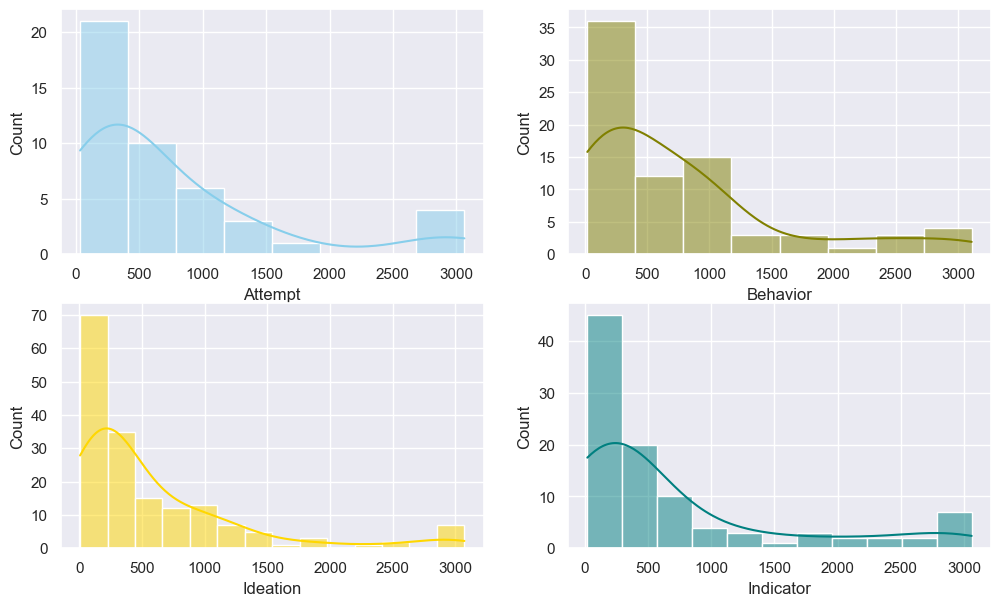
\includegraphics[width=\textwidth]{document_size_length_in_each_class.png}
\caption{Document size length in each class of suicidal category and samples frequency}
\label{reddit_cssrs_doc_len_freq}
\end{figure}

Text Data augmentation is applied here to increase the dataset size balancing samples of each class and synthetic dataset is prepared. Moreover, some standalone features are also provided belongs to specific category of suicide. Categorical features are mixed together shuffled and then chopped into fixed sized tokens and considered as sample sentences for specific category. This process continues until we found desired number of samples. Shuffling happens randomly and all the samples features only sentence and specific feature sentence are combined to prepare train classifier dataset. 

\subsection{Training Dataset}
In this research we have used dataset from \cite{gaur2019knowledge}. For training classifier in this research 2019's Gaur et. al \cite{gaur2019knowledge} Reddit C-SSRS dataset is used. Compared to the existing four-label classification scheme (no risk, low risk, moderate risk, and high risk), this dataset introduced 5 lavel classification of suicide 

\begin{enumerate}[label=(\roman*)]
\item Indicator - Indicates suicidal symptoms in the post
\item Ideation - Having suicidal Ideas 
\item Behavior - Having some suicidal symptoms Behavior
\item Attempt - Suicidal attempt in the post
\item Supportive - Someone shows empathy and condolence for a suicidal post
\end{enumerate}
Supportive category is not taken into account in the analysis section since supporting group does not belong to examined specimen individual. 

\subsection{Testing/Validation Dataset} 
For testing dataset is collected from kaggle. It is an opesource dataset publicly available collected from reddit website by a pushshift API contained suicide and depression category.  This publicly available Reddit datasets in Kaggle Website comprised of 232,074 post annotated for binary classification as suicidal or non-suicidal in \cite{aldhyani2022detecting} for detecting suicidal ideation. The dataset is a collection of posts from the "SuicideWatch" and "depression" subreddits of the Reddit platform. All posts that were made to "SuicideWatch" from Dec 16, 2008(creation) till Jan 2, 2021, were collected while "depression" posts were collected from Jan 1, 2009, to Jan 2, 2021. In this research trained classifier is applied to detect class on this two category. Main objective is to determine the suicide categories (indicator, ideation, behavior, attempt, supportive ) within this dataset. 

\section{Methodology}\label{sec2}
In several research papers reddit dataset has become a good estimator to determine depression and suicide. Reddit dataset is used as a test dataset for classifiers for this research because of its availability and open access. Here classifier is trained with the suicidal intensity determinant Twitter's dataset which is used to determine the depression intensity within a suicidal post. It  provides the suicidal risk classification dataset and has specific features belongs to specific category of suicidal risk. As test dataset for classification result Reddit's suicide vs depression dataset are chosen. Trained classifier, detects the suicidal risk within reddit post which contains depression vs suicide category. 

%\begin{figure}[h!]
%\centering
%\includegraphics[width=0.8\textwidth]{research diagram.jpeg}
%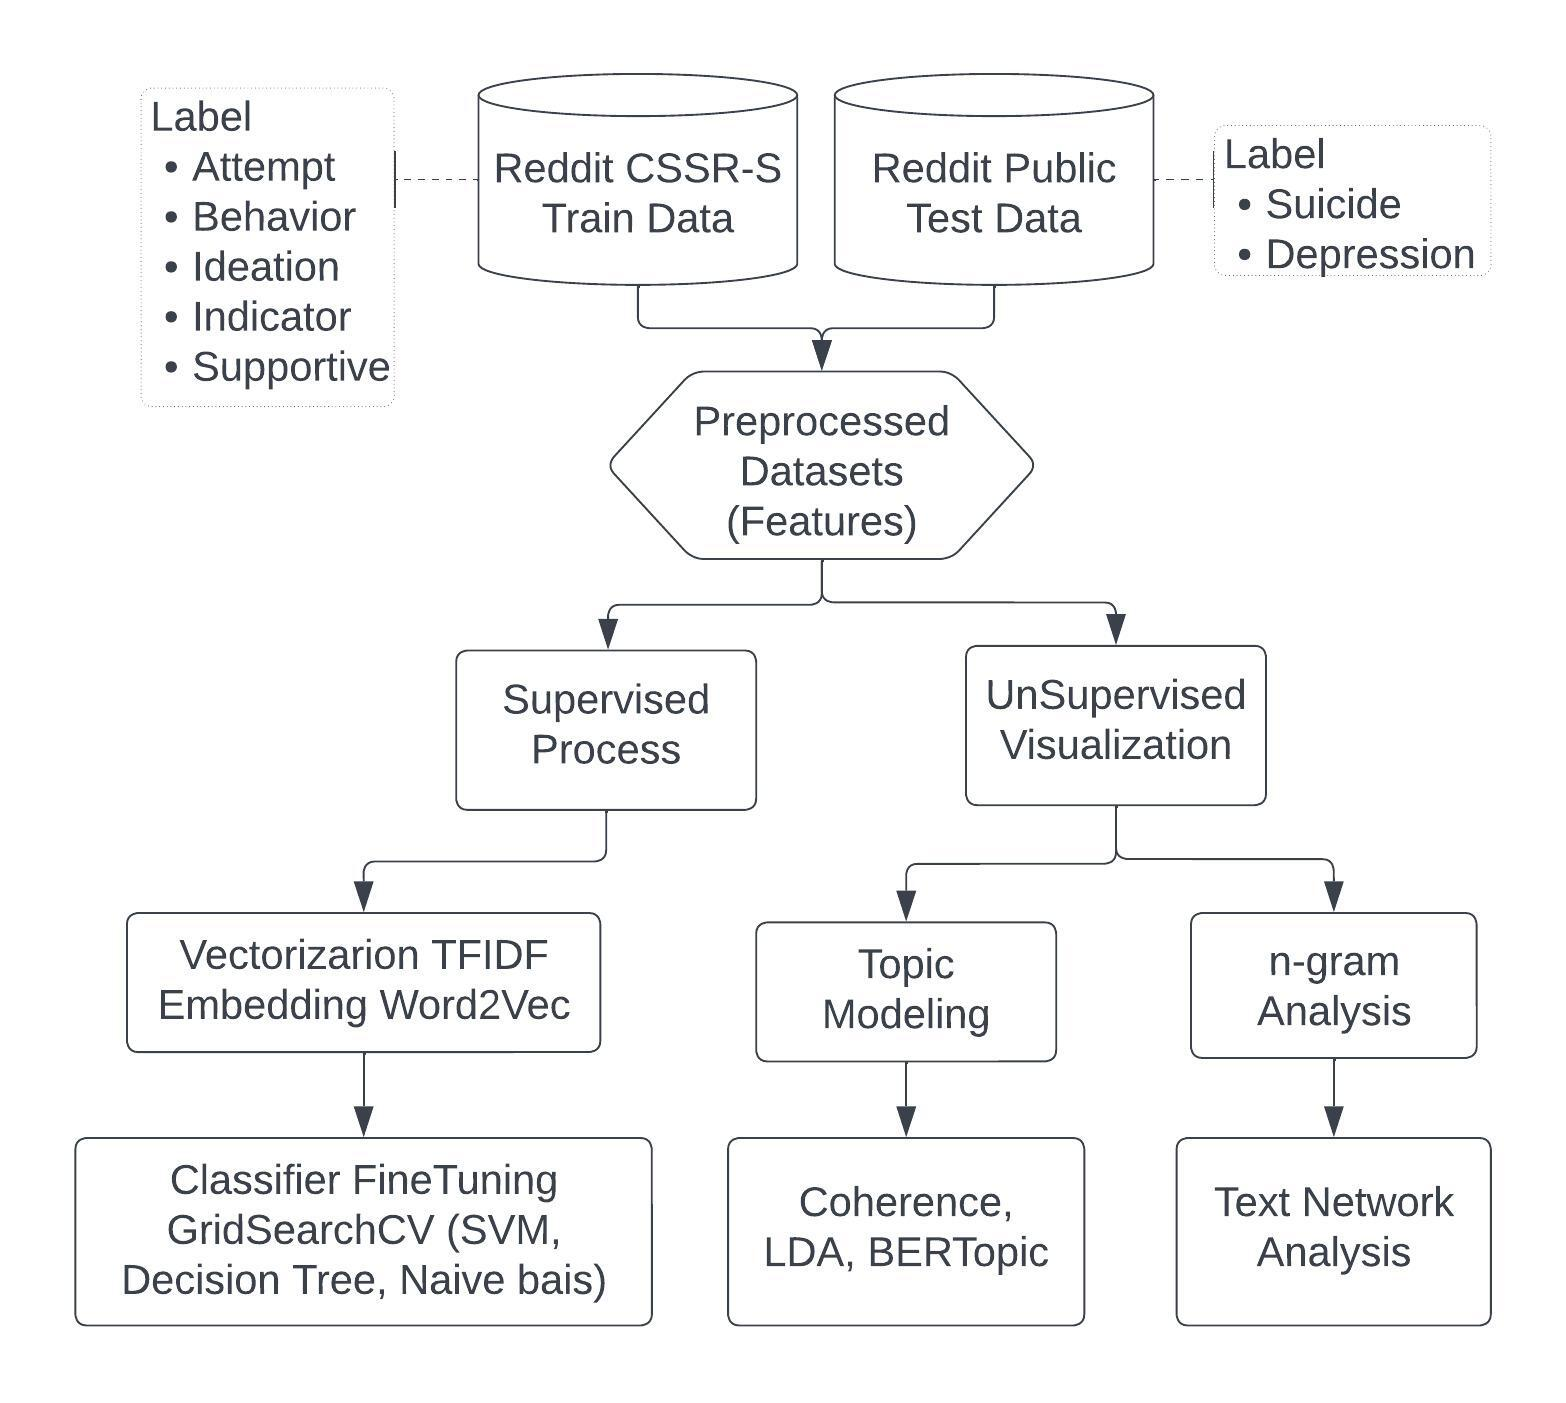
\includegraphics[width=0.8\textwidth]{res_diagram.jpeg}
%\caption{Research Methodology overview}
%\label{fig:res_diagram}
%\end{figure}

In this research dataset is pro-processed using the most common techniques of NLP mentioned in the section \ref{data_preprocessing}. We cleaned the dataset by removing unwanted characters, symbols and stop words. Then further pre-processing is conducted which are followed for standard data cleaning process for NLP task. Pre-processed dataset is converted to vector. Various vectorizer are used to convert the corpus into corresponding vector. Text is converted to meaningful feature vector then classifier is trained to determine depression degree within a suicidal post. Various vectorization methods are applied to get best possible outcomes. Then machine learning classifier is applied to estimate the class category. From the observed result statistical analysis explained the degree of depression within a suicidal post. In our analysis we used different classifiers to determine how suicide intensity is showed in depression vs suicide category dataset. Thereby we can infer degree of suicidal tendency within depression person's post. 

Hence, visualizing the result we can determine the suicidal tendency within depression post. Also, N-gram based analysis is conducted and frequency of Terms and connections of words or phrases are analyzed in this research scope. More often topic modeling clustering is used to determine latent topic and understand latent text network. From the network various facts can be revealed related to suicide and depression. This whole process is depicted in Figure \ref{fig:res_diagram}

\subsection{Data Processing and Models}
\subsubsection{Data Pre-processing}\label{data_preprocessing}
Social media dataset are mostly Text data which needs data pre-processing, cleaning, feature extraction and data mining related NLP tasks. NLP based text data contains noises such as: unnecessary quotes, special characters, punctuation etc. Moreover, morphological analysis is needed to retrieve root words followed by stemming, lemmatization. Then, sentences are divided into equal-length fragments, and null word padding is applied as needed. Words within a phrase are now referred to as tokens or features, and the dataset is shown as a corpus. Special features/tokens are further preprocessed and filtered using text data feature extraction tools and methods. Features are passed through a process in which features are converted to corresponding IDs and sentences which contains a series of IDs are represented a vector. The embedding is another term that is frequently used in relation to vector text analysis. Various Vectorization methods are present. Traditional vectorization method provide weights to terms/words mainly based on frequency of words within the sentence and documents, rather than its importance and contextual meaning. Also, how does a particular word or term create impact on the neighboring words is not taken into consideration, since these models does not have any prior knowledge of any words. Hence, various neural network based language models are proposed which are pretrained on massive amount of dataset. These models mainly carries weight which represents word to word relationships and most cases can provide contextual meaning of given sentence based on pretrained dataset knowledge. Deep learning models recently showed remarkable achievements in this case representing corresponding knowledge.

\subsection{Latent Dirichlet Allocation (LDA)}
\label{lda_mdel}
LDA model \cite{jelodar_latent_2019, gupta_pan_lda_2021, pichardo_lagunas_svd_lda_2015, selvi_classification_2019} considers documents are mixes of topic, and each topic is a distribution over words. The objective is to derive the hidden topic assignments and the topic-word distributions that most effectively describe the observed documents. The goal of LDA is to uncover these latent topics from a collection of documents without needing any prior labeling or categorization of the content. An expression for the joint distribution of the LDA model is described below:  
\begin{equation}
P(\theta_d,z,w\|\alpha,\beta)=P(\theta_d\|\alpha)\prod^N_{n=1}P(z_{d,n}\|\theta_d)P(w_{d,n}\|z_{d,n},\beta)
\end{equation}
Where $w_{d,n}$ the $n_{th}$ word in document $d$, $z_{d,n}$ the topic assigned to the $n_{th}$ word in document $d$, $\alpha,\beta$ are the Dirichlet LDA model parameters. controls per-document topic distribution, and per topic word distribution. $\theta_d$ represent the topic distribution. $P(\theta_d \| \alpha)$ Dirichlet 
distribution representing the document-topic distribution, $P(z_{d,n}\|\theta_d)$ is the word topic assignment for the $n_{th}$ word in document $d$, $P(w_{d,n}\|z_{d,n},\beta)$ is the distribution representing the observed word given a topic. We have chosen LDA for baseline statistical topic modeling tool. However, how many topics are ideal it is needed to determine and also topic modeling quality needs to measure.

\subsubsection{Topic models comparative analysis}
While some variations of LDA, Mallet LDA is considered for large corpus processing and analysis \cite{vayansky2020review, abdelrazek2022topic, Comparison_Topic_Modeling_Algorithms}. It focuses on scalability, If large corpus needs to analyze, Mallet LDA might be more suitable. LDA in general can still be efficiently applied to moderately sized corpora. Analyzing topics within the context of metadata, STM could be a better fit. Hierarchical Dirichlet Process (HDP) can be useful when we cannot guess the number of topics in advance. In \cite{Comparison_Topic_Modeling_Algorithms} LSI, NMF and LDA are compared in terms of coherence and similarity measures for social media dataset and in their analysis NMF is observed most effective measures. However, as a baseline model LDA is often considered one of the most prominent choices. In this study Textbook corpus is divided into lessons which is a mixture of topics and using LDA expecting to determine which word in the lesson belong to Lesson\textquotesingle s topics. LDA produces interpretative results for exploratory topic analysis. The identified topics are represented as distributions over words, making it easy to assign meaningful labels to topics. Provided by most of the libraries and tools, making it easy to implement and can be integrated into existing workflows. Hence, LDA serves as a solid baseline for topic modeling tasks.  

\subsubsection{Optimal Topics with Coherence}  
Coherence score measure how coherent or interpret the words in that topic and estimates number of topic clusters \cite{mimno2011optimizing}. Coherence score assess the quality of the topics produced by LDA and ensures that the topics generated are statistically significant. Coherence \(C_{topic}\) can be expressed as follows  
\begin{equation}
C_{topic}=\sum^N_{i=1} \frac{1}{N(N-1)}\sum^i_{j=1} PMI(w_i,w_j)
\end{equation}
Where, \(PMI\left( w_{i},w_{j} \right)\) represent pointwise mutual information statistical association between two words occurring together. PMI score indicates that the two words are more closely related within a topic. \(PMI\left( w_{i},w_{j} \right)\) can expressed as  
\begin{equation}
\(PMI\left( w_{i},w_{j} \right) = \log\frac{P\left( w_{i},w_{j} \right)}{P\left( w_{i} \right)P\left( w_{j} \right)}\)
\end{equation}

where \(P\left( w_{i},w_{j} \right)\) is joint probability of occurrence of words \(w_{i}\) and \(w_{j}\).  To calculate the coherence score gensim library provides range of options such as \(u_{mass},c_{v},c_{uci},c_{npmi}\). \(u_{mass}\) and \(c_{v}\)These two methods are most popular. For given topic with words \(\{ w_{1},w_{2},w_{3},\ldots..,w_{n}\}\) a fixed context window size is provided (default size 10 words) then coherence score is calculated using an equation \(\sum_{j = 1}^{i}{PMI}\left( w_{i},w_{j} \right)\) which provides negative coherence score. \(c_{v}\) can be expressed as  
\begin{equation}
\(c_{v} = \frac{1}{N(N - 1)}\sum_{j = 1}^{i}{similarity\left( w_{i},w_{j} \right)}\)
\end{equation}
in which \(similarity\left( w_{i},w_{j} \right)\) represent the pairwise similarity between terms based on \(PMI\left( w_{i},w_{j} \right)\) scores. \(c_{v}\) provides a positive coherence score. Higher coherence values (higher than 0.5) indicate that the topics are moderately coherent and representative of meaningful themes within the text data.


\section{Feature exploration}
Word cloud is showed in figure \ref{redditdist_twitterdist_wordcloud} to depict each category and influence of dominant keywords based on frequency.  

\begin{figure}[h!]
\centering
\begin{subfigure}{0.45\textwidth}
    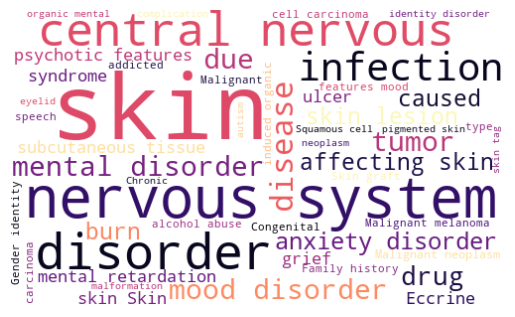
\includegraphics[width=\textwidth]{indicator_word_cloud.png}
    \caption{Indicator category word high impact words are anxiety, disease, disorder, nervous etc}
    \label{redditdist}
\end{subfigure}
\hfill
\begin{subfigure}{0.45\textwidth}
    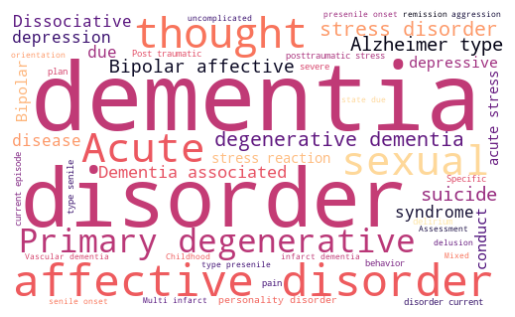
\includegraphics[width=\textwidth]{Ideation_word_cloud.png}
    \caption{Ideation category word cloud high impact words are dementia, affective disorder, stress, bipolar personality}
    \label{twitterdist}
\end{subfigure}      
\centering
\begin{subfigure}{0.45\textwidth}
    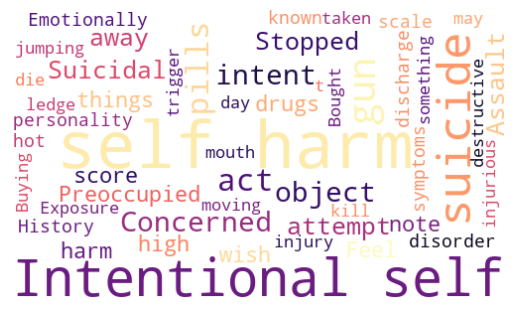
\includegraphics[width=\textwidth]{Behavior_word_cloud.png}
    \caption{Behavior category word cloud high impact words are self-harm, suicidal, intentional etc.}
    \label{redditdist}
\end{subfigure}
\hfill
\begin{subfigure}{0.45\textwidth}
    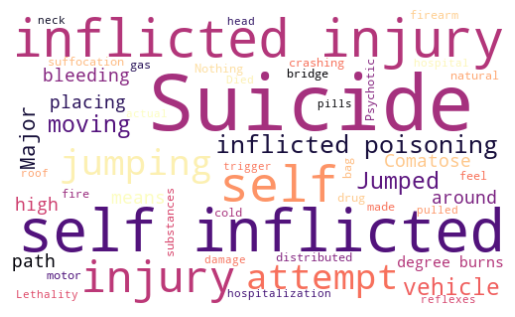
\includegraphics[width=\textwidth]{Attempt_word_cloud.png}
    \caption{Attempt category word cloud high impact keywords suicide, attempt, inflicted injury etc.}
    \label{twitterdist}
\end{subfigure}   
\caption{Train Reddit C-SSRS dataset word cloud distribution represents that there are overlapping features between Indicator with Ideation and Behavior with Attempt categories}
\label{redditdist_twitterdist_wordcloud}
\end{figure}

Document length frequency and token distribution is depicted in Figure \ref{redditdist_twitterdist_together}. From the frequency distribution we can see some of the document sizes are very large. Hence, during the training process we chopped the sentences into multiple sentences keeping the label same. 

\begin{figure}[H]
\centering
\begin{subfigure}{0.45\textwidth}
    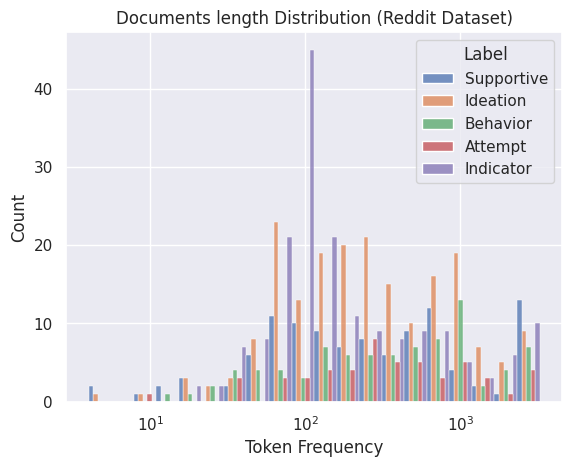
\includegraphics[width=\textwidth]{reddit_dist.png}
    \caption{Reddit dataset distribution}
    \label{redditdist}
\end{subfigure}
\hfill
\begin{subfigure}{0.45\textwidth}
    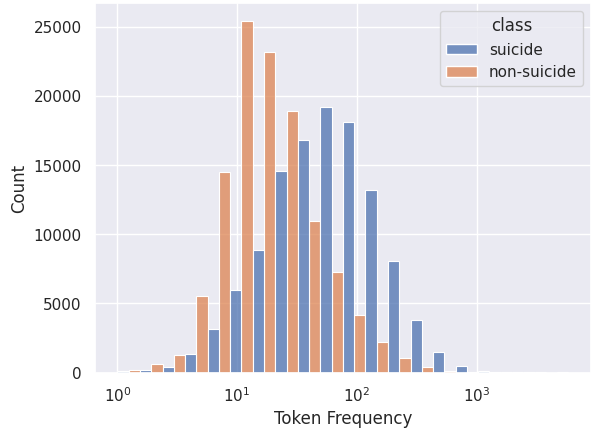
\includegraphics[width=\textwidth]{twitterdist.png}
    \caption{Twitter dataset distribution}
    \label{twitterdist}
\end{subfigure}       
\caption{Train and Test dataset Twitter and Reddit dataset distribution}
\label{redditdist_twitterdist_together}
\end{figure}

\subsection{N-gram Analysis}
\subsubsection{Uni-gram}
Dataset is split into separate tokens after preprocessing and uni-gram generated. Based on frequency of words wordcloud is generated from these unigrams. Frequency based comparison between two categories is conducted for depression and suicide for Test dataset in Figure \ref{features_vis_pro_exp}. Main objective was to get top ranked words from Depression and Suicide corpus. After experiments we have seen There are similarities between the top ranked words those are occurring frequently. They tend to use slang and abusive terms compared to suicidal attempt thinking people. Rather suicidal depressed people want to share their thoughts with others using longer post. However, it does not reveals any clues in terms of hypothetical relationships between the two category. It is difficult find pattern in which we can determine the depression and suicidal thought. So far we found some pattern 
\begin{enumerate}
\item short statements likely to be more depression category
\item Depressive statements tend to have slang
\item Suicidal thinking people’s post having very high frequency of “kill” “die” these type of words or phrases.
\end{enumerate}

\begin{figure}[H]
\centering
\begin{subfigure}{0.45\textwidth}
    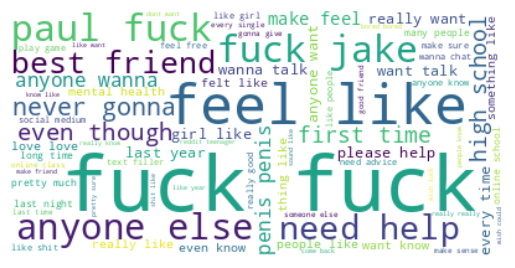
\includegraphics[width=\textwidth]{dep_wordcloud.png}
    \caption{Wordcloud in Depression category}
    \label{fig:first}
\end{subfigure}
\hfill
\begin{subfigure}{0.45\textwidth}
    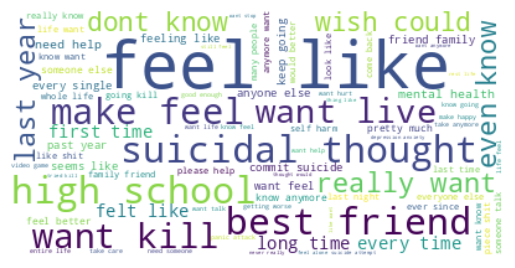
\includegraphics[width=\textwidth]{sui_wordcloud.png}
    \caption{Wordcloud in Suicide category}
    \label{fig:second}
\end{subfigure}
\hfill
\begin{subfigure}{0.8\textwidth}
    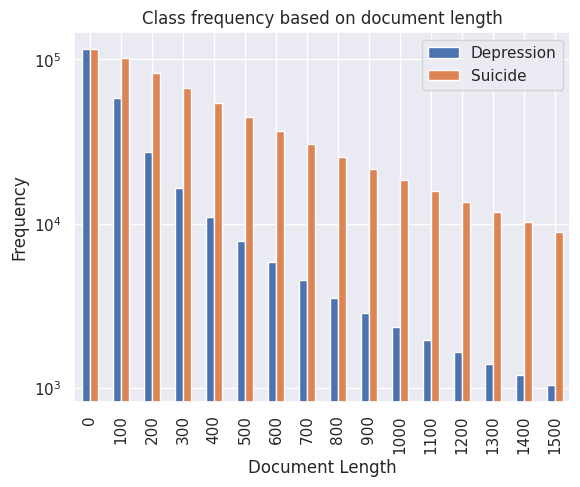
\includegraphics[height=7.5cm, width=\textwidth]{doc_len.png}
    \caption{Class frequency in different Document Length}
    \label{fig:second}
\end{subfigure}        
\caption{Dataset features visualization and properties exploration}
\label{features_vis_pro_exp}
\end{figure}

To understand the term occurring frequently in two different classes scatterplot library is used for visual analysis. From the above two scenario we can see that there is a pattern that people used to say more slang and abusive words when they are depressed. It is also interesting that there are many words have high frequency such as depression or depressed but belongs to suicide class. One important fact is revealed here is that we can see although suicide, suicidal these words has high frequency in Suicide class but depression, depressed also occurred in parallel with high frequency. Here several experiments can be conducted for exploratory analysis with scattertext library for terms significance. However, this library is computationally heavy for larger dataset for visualization. Another drawbacks is this library have significant focus on the terms based analysis. We have used simple vectorization methods by which we can have greater control on dataset and experiments code. 

\subsubsection{Bi-gram}
First unigram is computed and analyzed then bigram is calculated for both categories. The bigram frequency showed there are some common terms like “mental health”, “feel like”, “make feel”, “high school” etc showed high occurrences in the dataset. Hence, we started to understand its pattern in the corpus. For analysis we have considered ['high school', 'mental health', 'best friend', 'feel like', 'really want', 'suicide thought', 'friend family'] these bi-grams and wanted to explore its surrounding context for each category. We called this special bigrams since it showed importance in the suicidal and depression both categories appeared highly frequent matter. We want to analyze how these words have impact with its neighboring words. 

To explore the impact of special bi-grams on the samples, special bi-gram terms containing samples are filtered from dataset. After that using lebel encoder bigrams are encoded as integers and then chord diagram is generated  depicted in Figure \ref{Bigram_features_exp} to find meaningful relationship within the samples between the bigram features.  


\begin{figure}[H]
\centering
\begin{subfigure}{0.8\textwidth}
    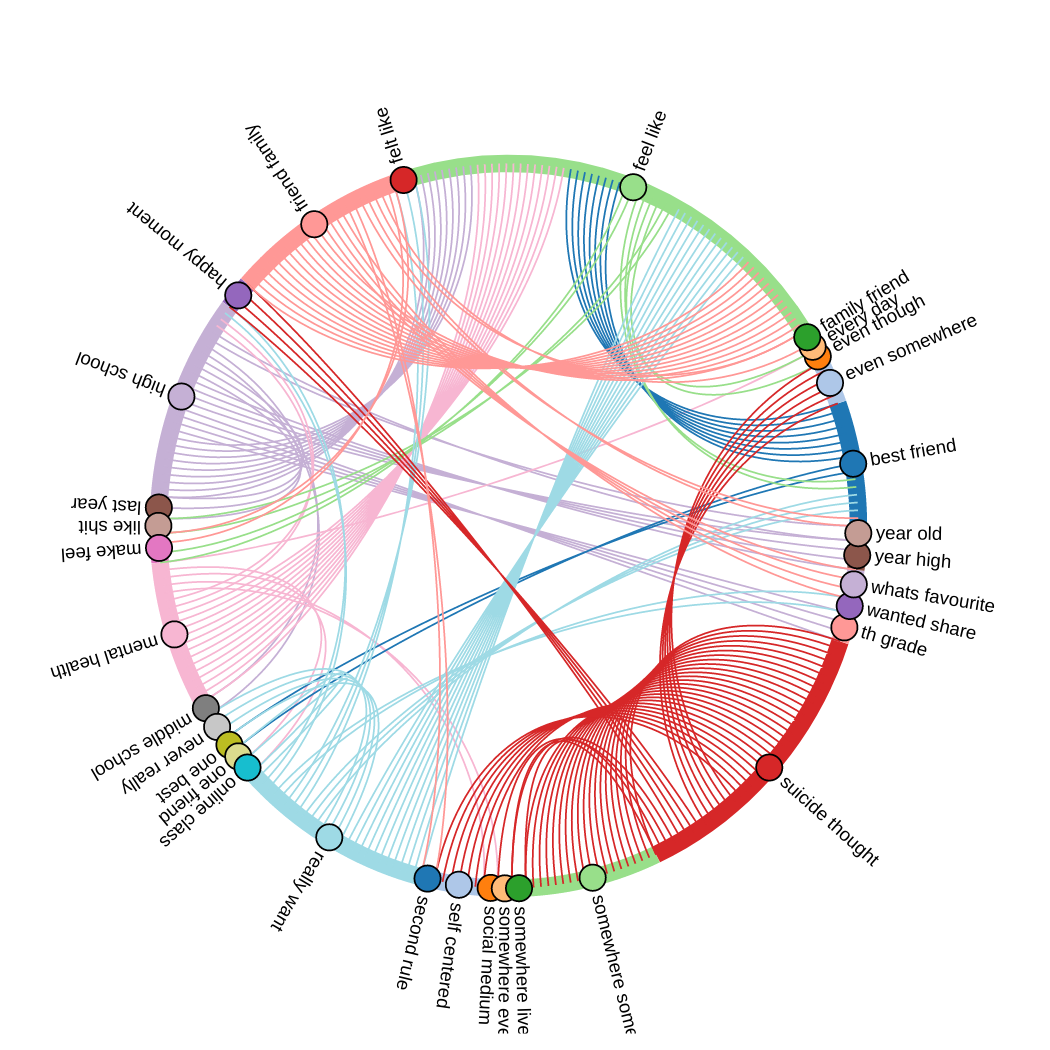
\includegraphics[width=\textwidth]{dep_chord.png}
    \caption{Depression Chord diagram}
    \label{fig:first}
\end{subfigure}
\hfill
\begin{subfigure}{0.8\textwidth}
    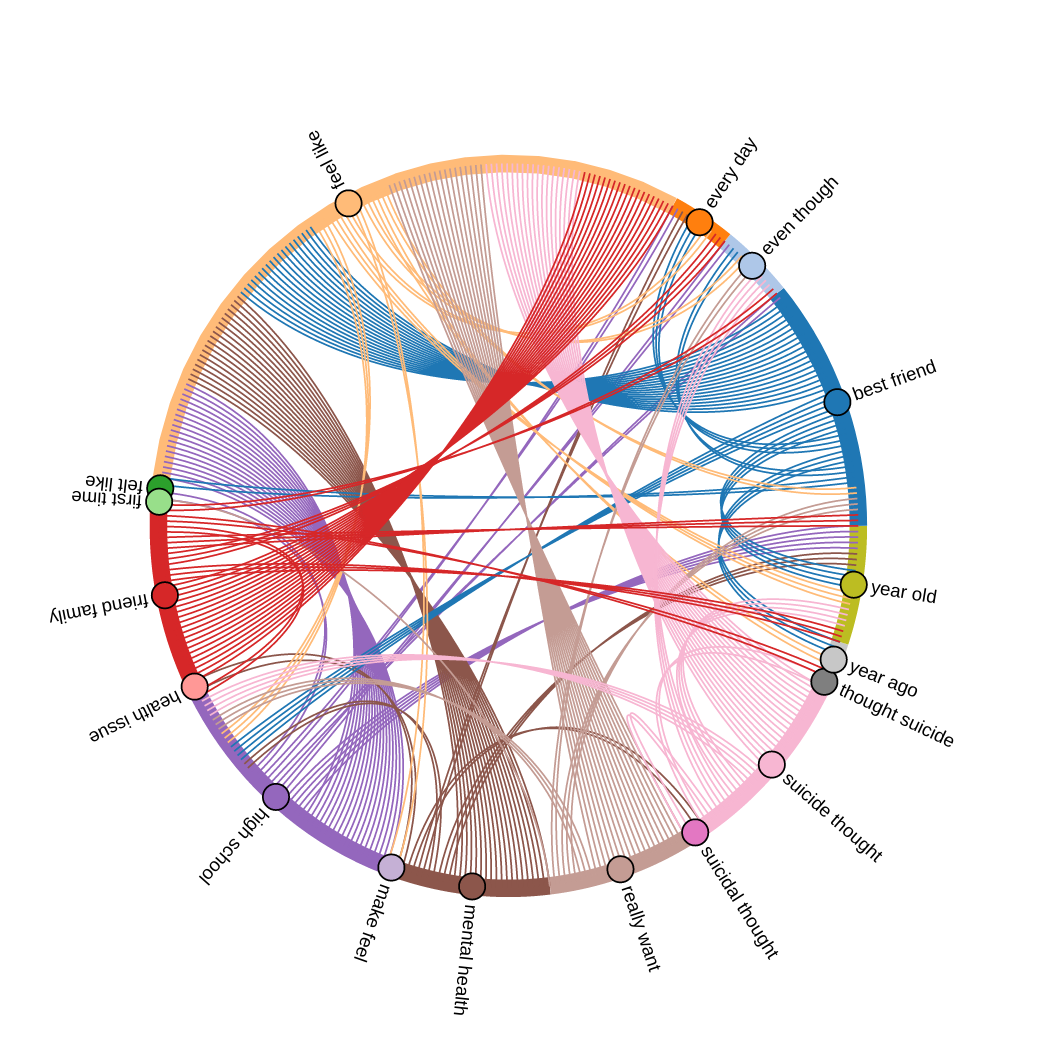
\includegraphics[width=\textwidth]{suicide_chord.png}
    \caption{Depression Chord diagram}
    \label{fig:second}
\end{subfigure}        
\caption{Bi-gram features relation exploration}
\label{Bigram_features_exp}
\end{figure}


From this two chord diagram interesting sentence can be inferred. 

\begin{table}[h]
\begin{center}
\begin{flushleft}
\caption{Inference from chord diagrams}\label{tab1}%
\begin{tabular}{|l|p{6cm}|}
\toprule
\textbf{Depression} & \textbf{Suicide} \\
\midrule
self centered person is depressed & have mental health issue \\
having suicidal thought & share though with friends (high school friends, Best friends, family members) \\
want to go somewhere to live & having suicidal thoughts \\
spend happy moments & Friend family make feel better \\
\bottomrule
\end{tabular}
%\footnotetext{Inference from chord diagrams}
\end{flushleft}
\end{center}
\end{table}

Tri-grams or above did not reveals much meaning information, mostly does convey some meaningful information and therefore excluded for further experimental consideration. 



\section{Exploratory analysis using Topic Modeling}
 Different techniques have been developed to perform topic modeling in the unsupervised topic modeling domain of Natural Language Processing (NLP), having their own strengths and limitations \cite{vayansky2020review, abdelrazek2022topic, yi2009comparative}. Apart from LDA, Mallet LDA, Structural Topic Model (STM), Hierarchical Dirichlet Process (HDP), Non-Negative Matrix Factorization (NMF), Latent Semantic Analysis (LSA) etc are also prevailing and can be considered for comparative research study.

\subsubsection{Dominant Keywords Determination}



\subsubsection{LDA model coherence to determine optimal topic}
\begin{figure}[h!]
\centering
\begin{subfigure}{0.45\textwidth}
    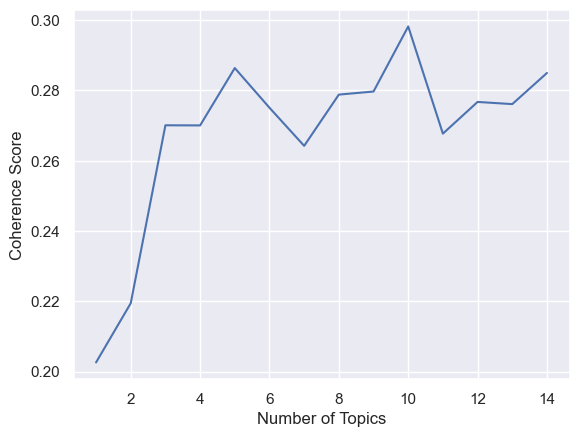
\includegraphics[width=\textwidth]{cv_indicator.png}
    \caption{Indicator category word cloud}
    \label{redditdist}
\end{subfigure}
\hfill
\begin{subfigure}{0.45\textwidth}
    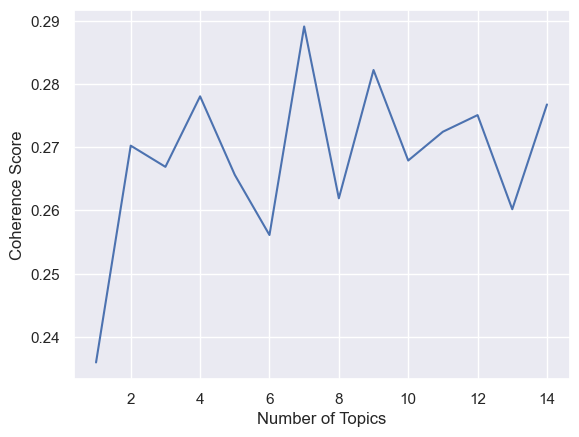
\includegraphics[width=\textwidth]{cv_ideation.png}
    \caption{Ideation category word cloud}
    \label{twitterdist}
\end{subfigure}      
\centering
\begin{subfigure}{0.45\textwidth}
    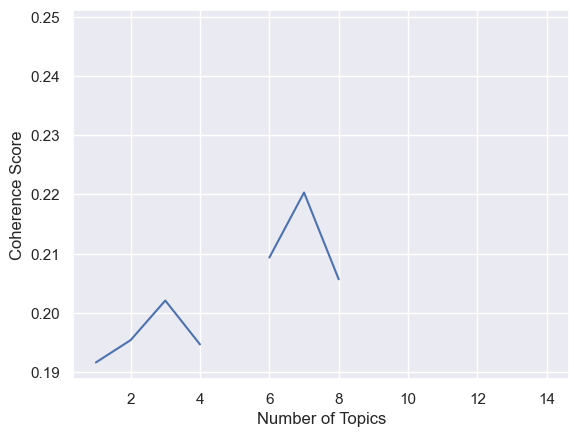
\includegraphics[width=\textwidth]{cv_behavior.png}
    \caption{Behavior category word cloud}
    \label{redditdist}
\end{subfigure}
\hfill
\begin{subfigure}{0.45\textwidth}
    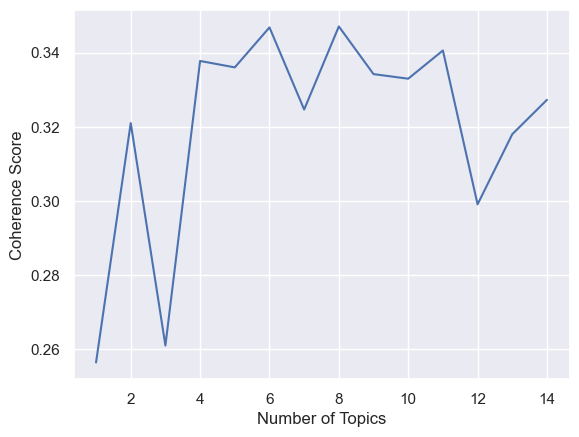
\includegraphics[width=\textwidth]{cv_attempt.png}
    \caption{Attempt category word cloud}
    \label{twitterdist}
\end{subfigure}   
%\caption{Train Reddit C-SSRS dataset word cloud distribution}
\label{redditdist_twitterdist}
\end{figure}


\subsubsection{Relative importance vs term frequency}
Relative importance is measured using LDA model. Then depicted in figure \ref{}. 
%\begin{figure}[h!]
%\centering
%\begin{subfigure}{0.45\textwidth}
%    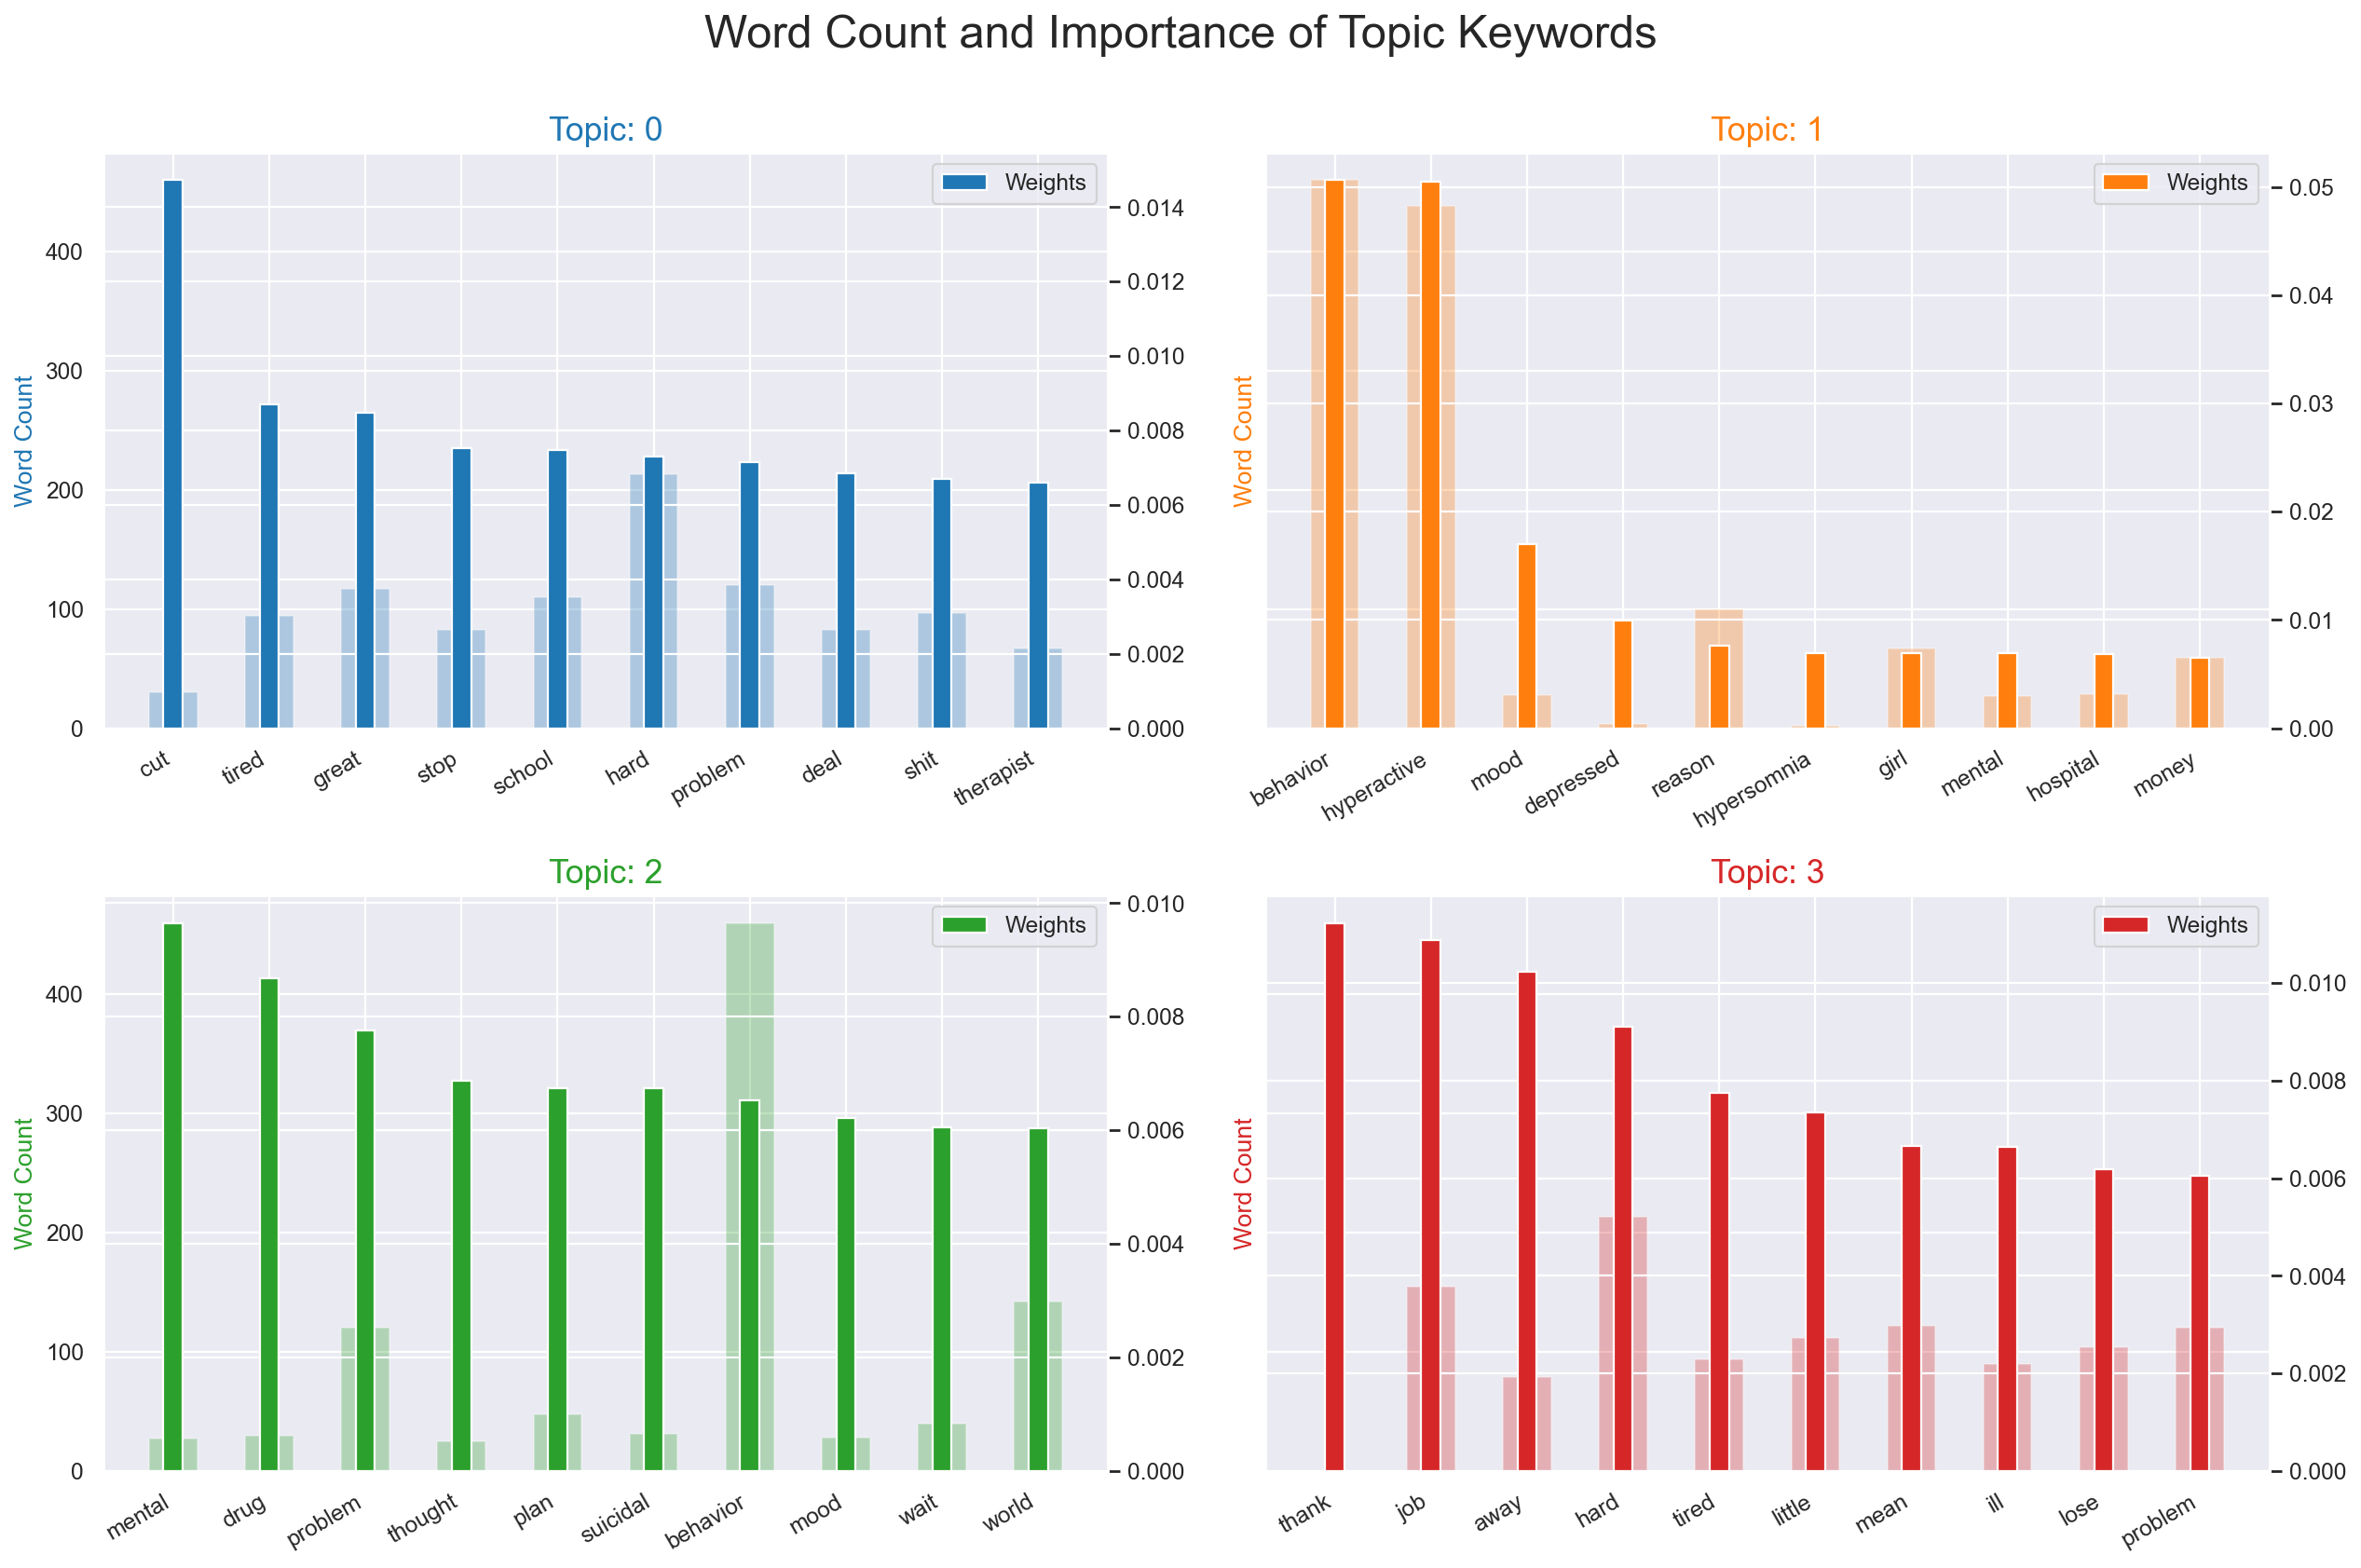
\includegraphics[width=\textwidth]{indicator_weight_relative_imp.png}
%    \caption{Indicator category word cloud}
%    \label{redditdist}
%\end{subfigure}
%\hfill
%\begin{subfigure}{0.45\textwidth}
%    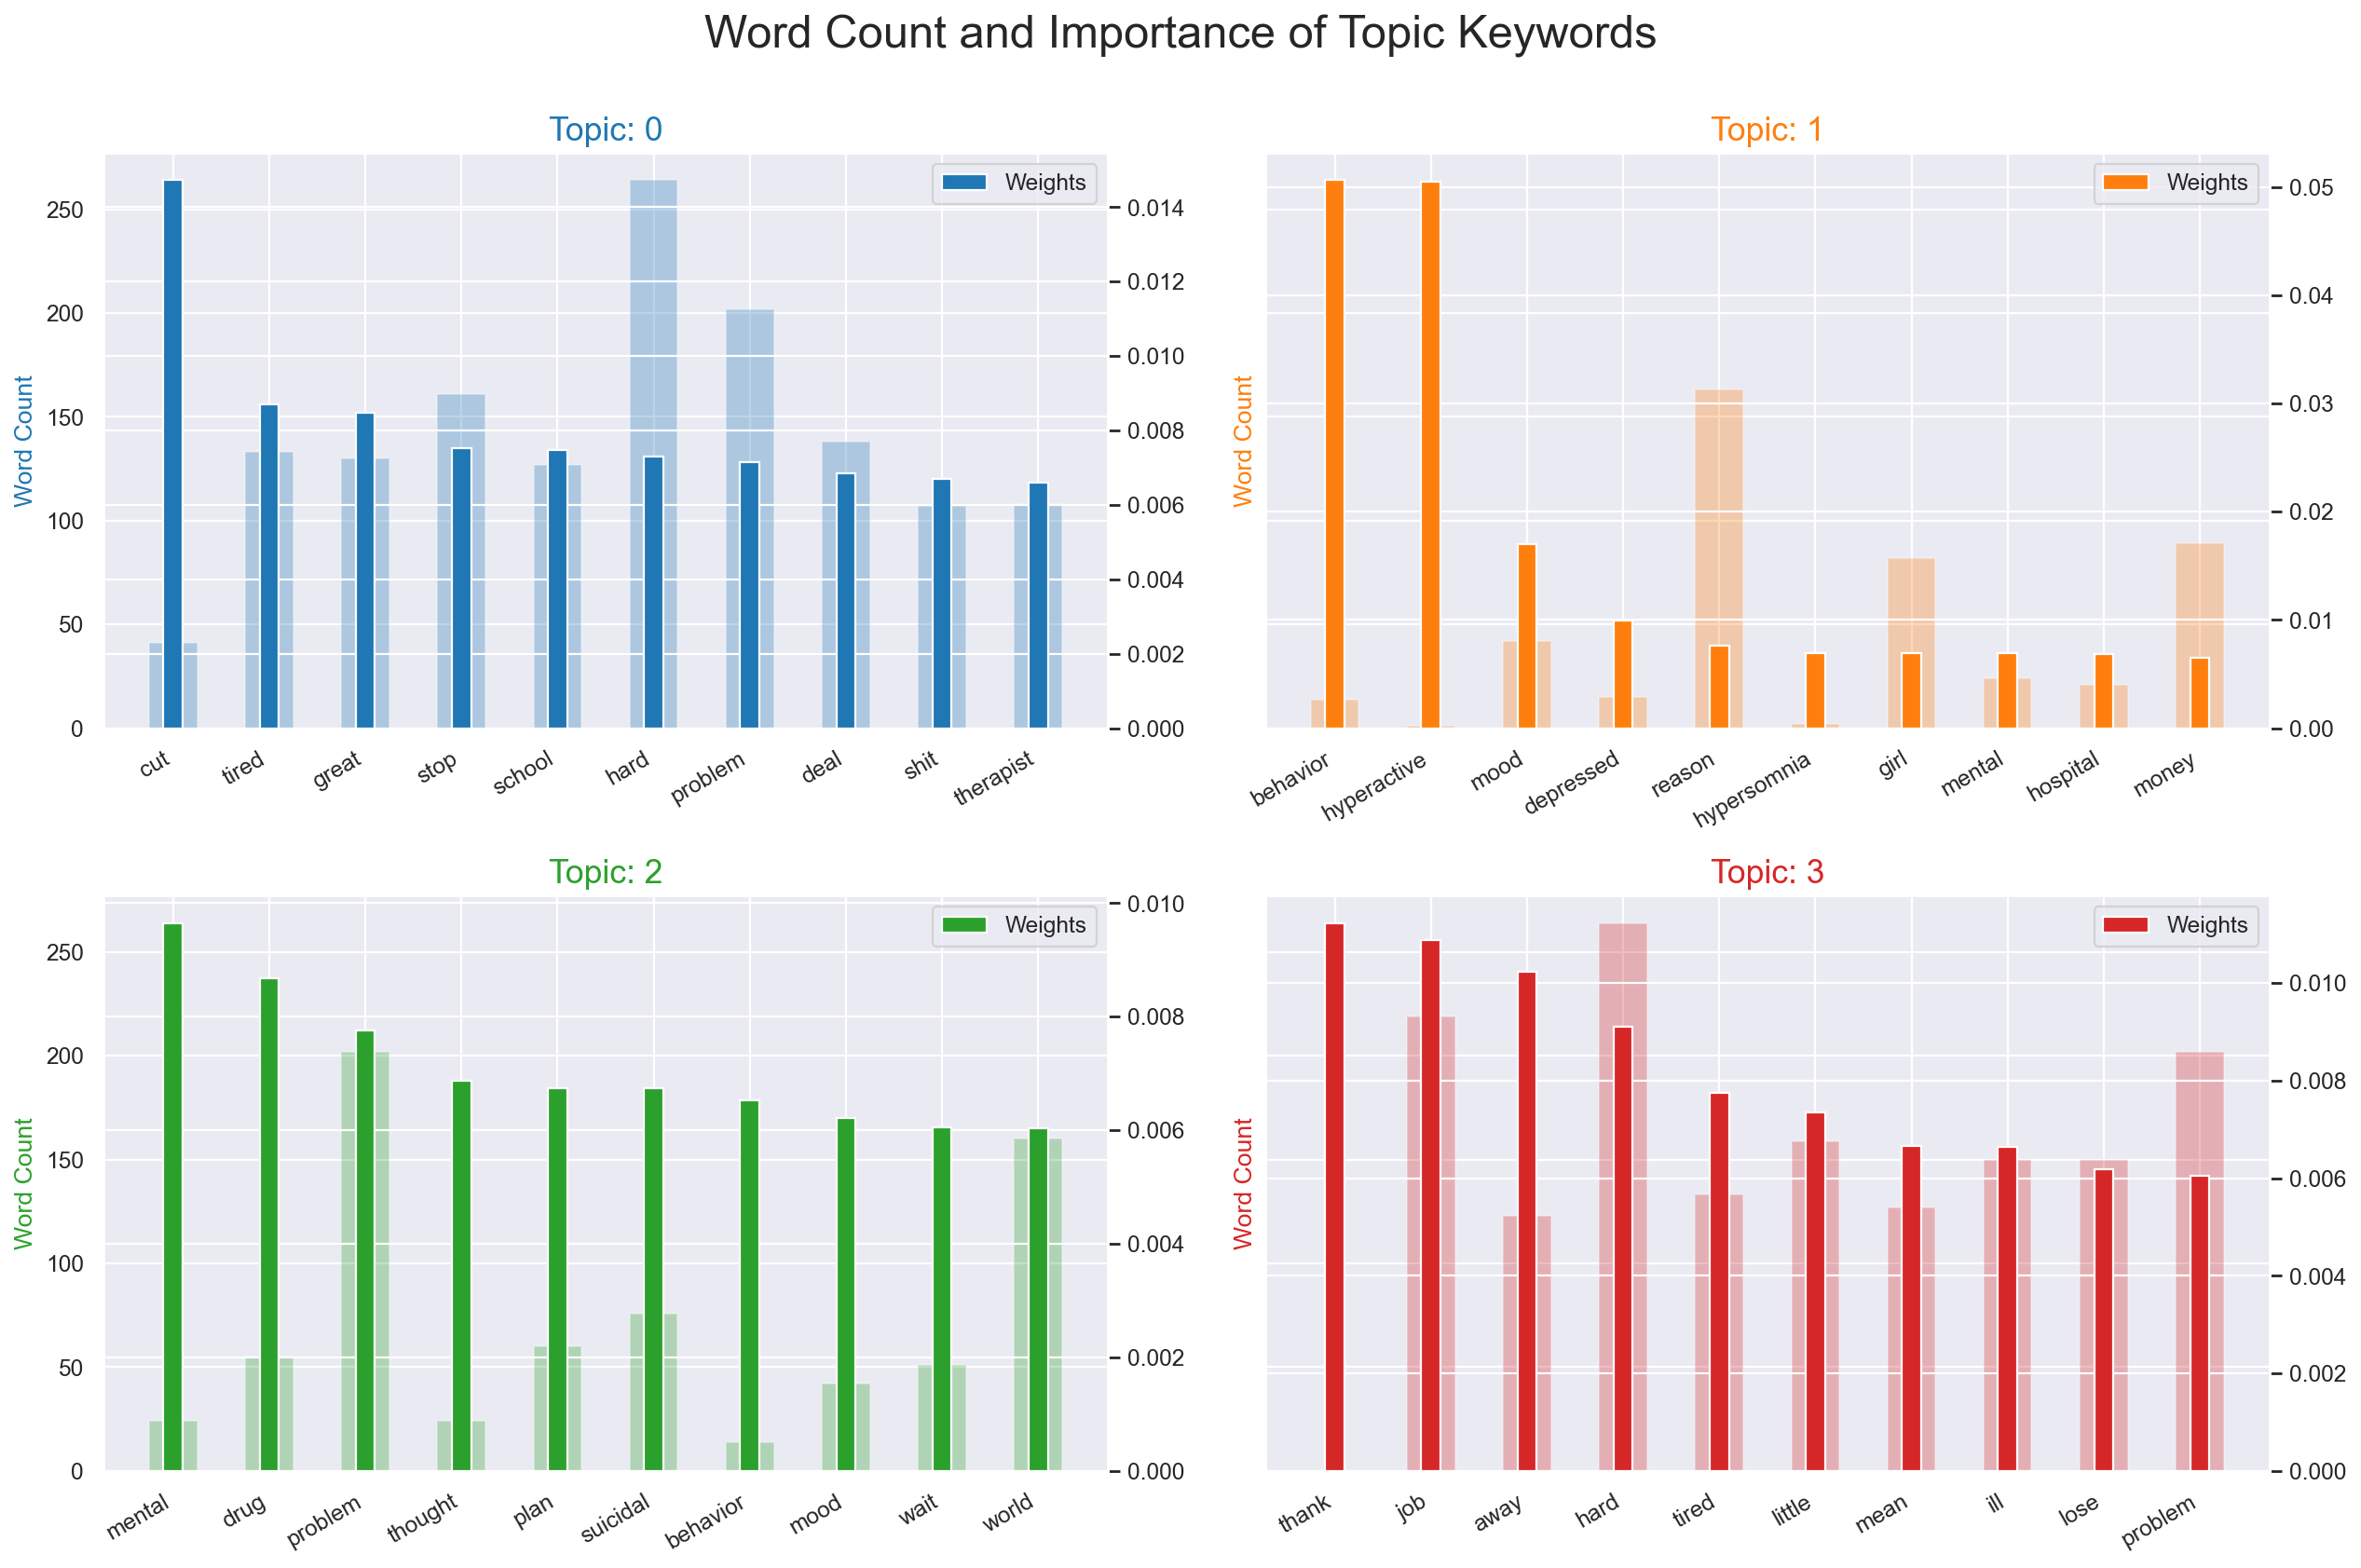
\includegraphics[width=\textwidth]{ideation_weight_relative_imp.png}
%    \caption{Ideation category word cloud}
%    \label{twitterdist}
%\end{subfigure}      
%\centering
%\begin{subfigure}{0.45\textwidth}
%    \includegraphics[width=\textwidth]{behavior_weight_relative_imp.png}
%    \caption{Behavior category word cloud}
%    \label{redditdist}
%\end{subfigure}
%\hfill
%\begin{subfigure}{0.45\textwidth}
%    \includegraphics[width=\textwidth]{attempt_weight_relative_imp.png}
%    \caption{Attempt category word cloud}
%    \label{twitterdist}
%\end{subfigure}   
%%\caption{Train Reddit C-SSRS dataset word cloud distribution}
%\label{redditdist_twitterdist}
%\end{figure}


\begin{figure}[H]
    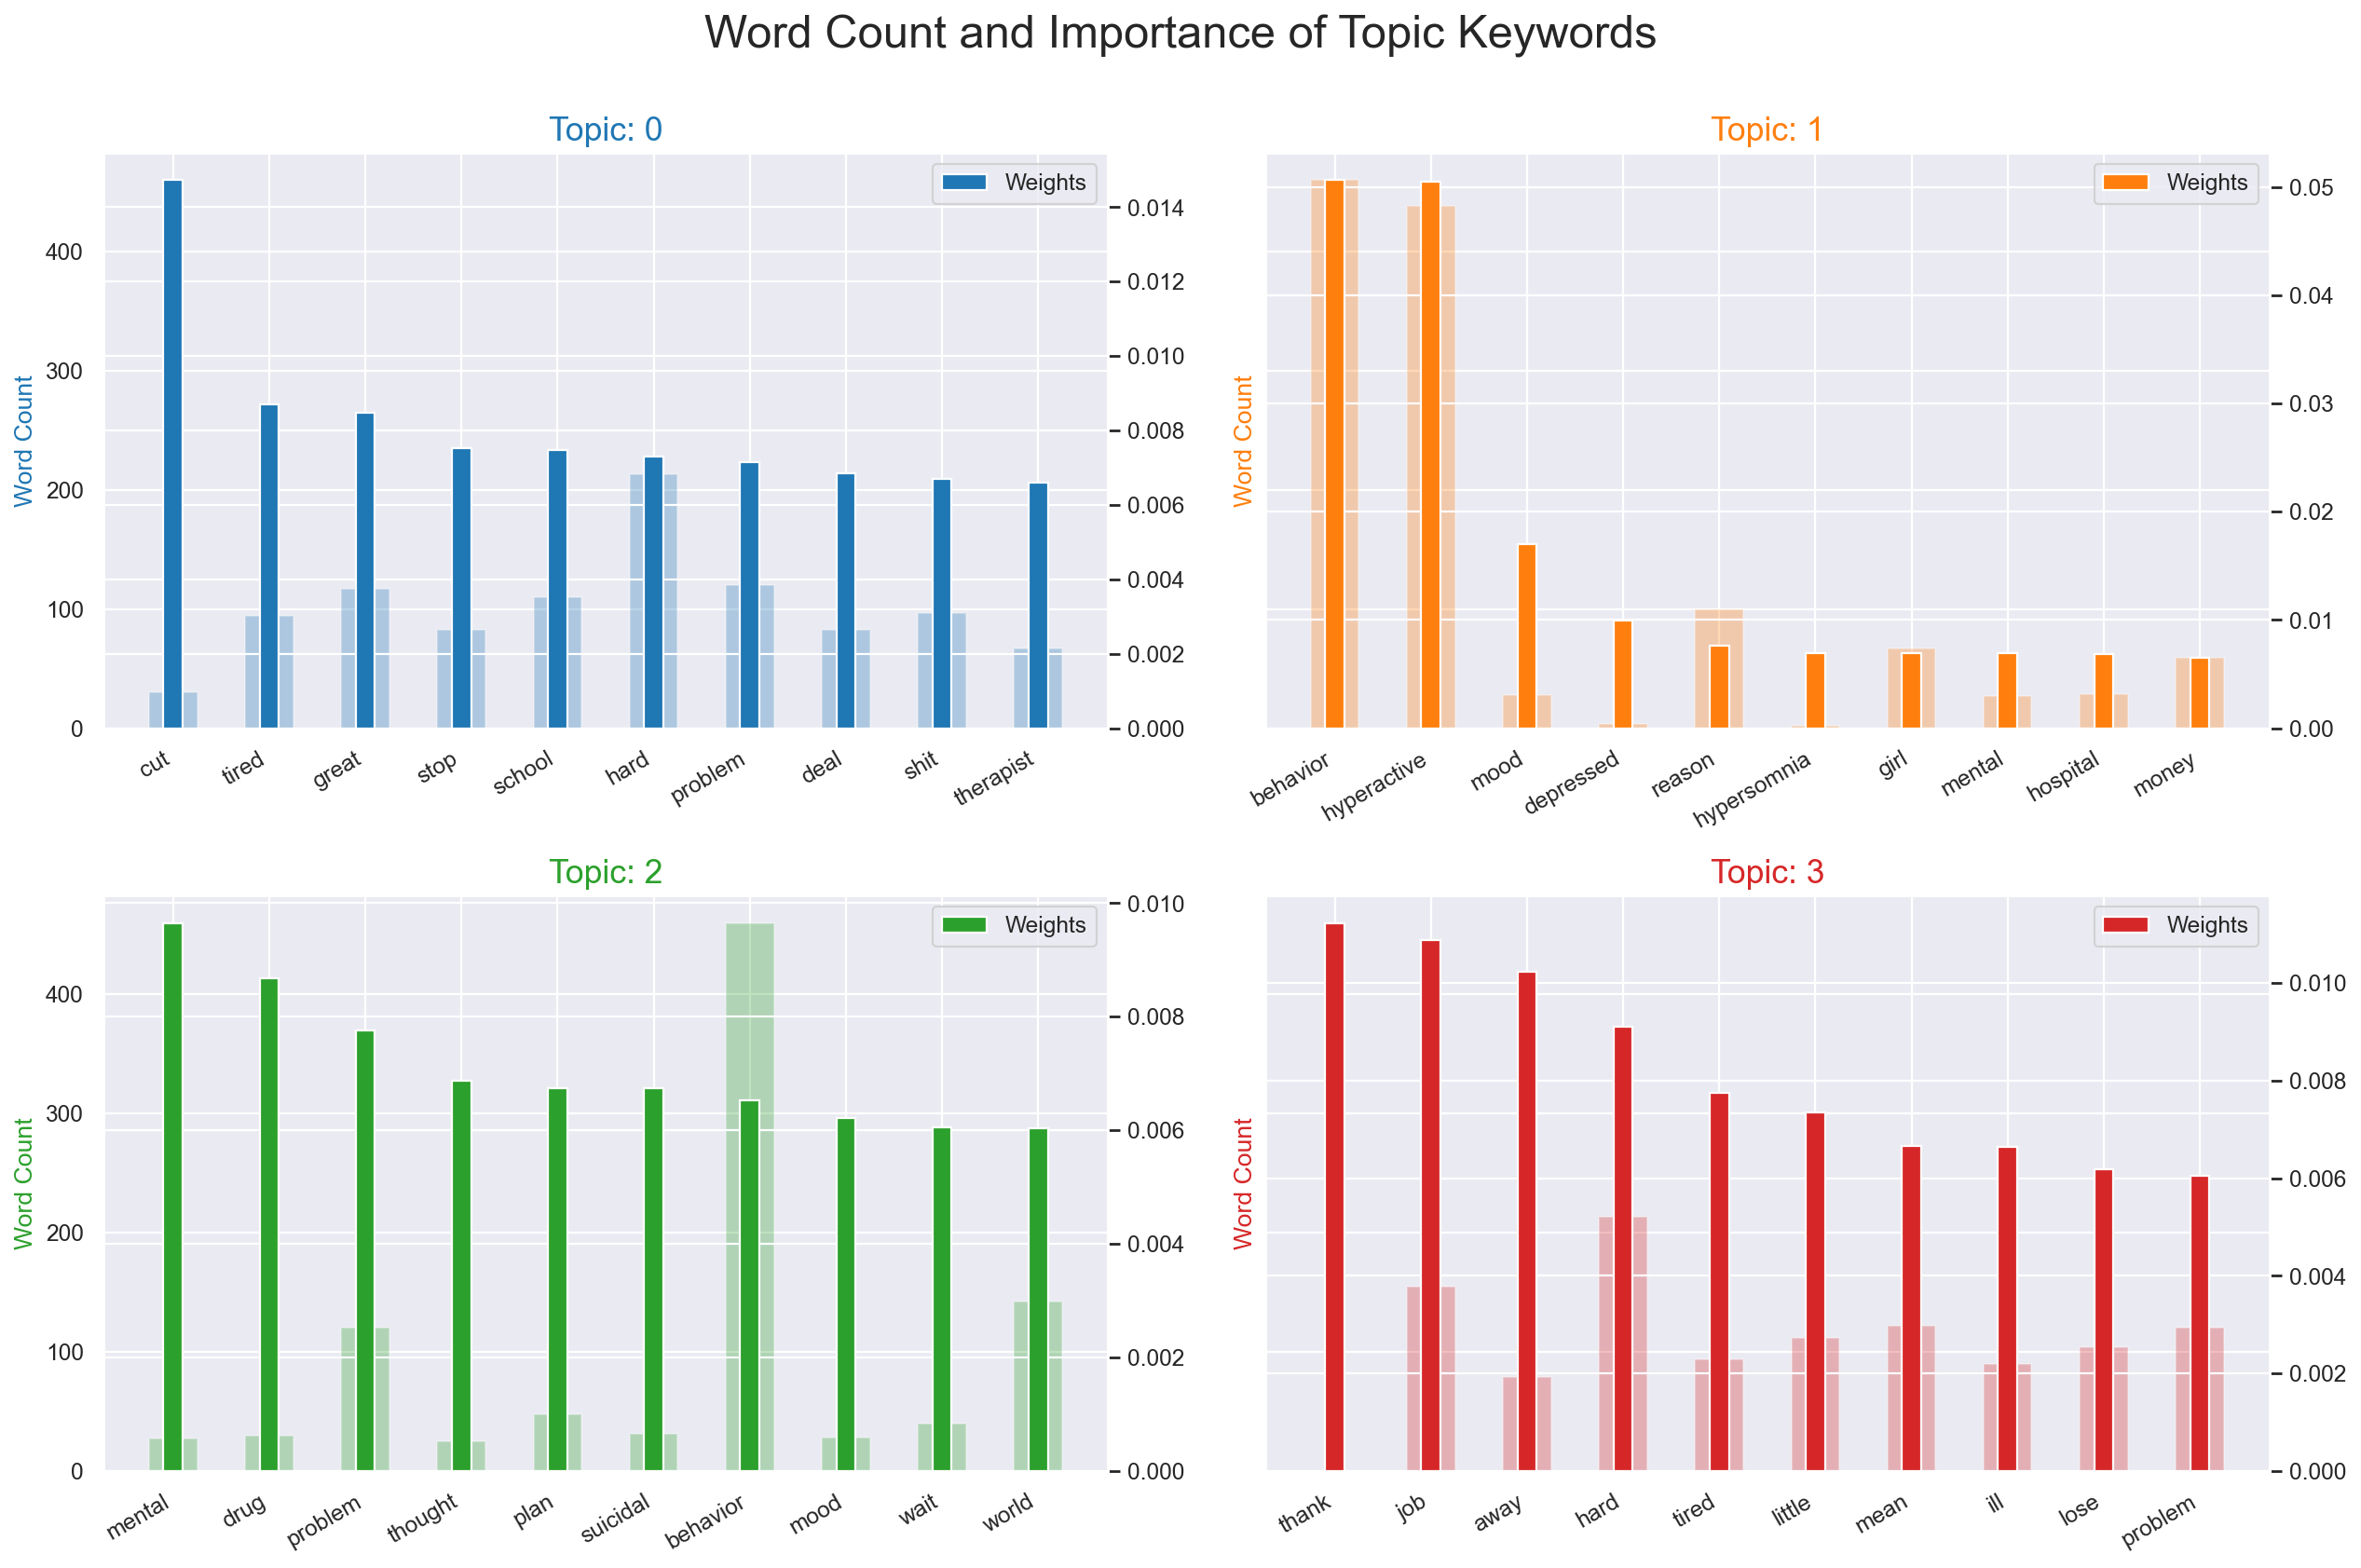
\includegraphics[width=\textwidth]{indicator_weight_relative_imp.png}
    \caption{Indicator category frequency vs LDA based relative Importance}
    \label{redditdist}
\end{figure}


\begin{figure}[H]
    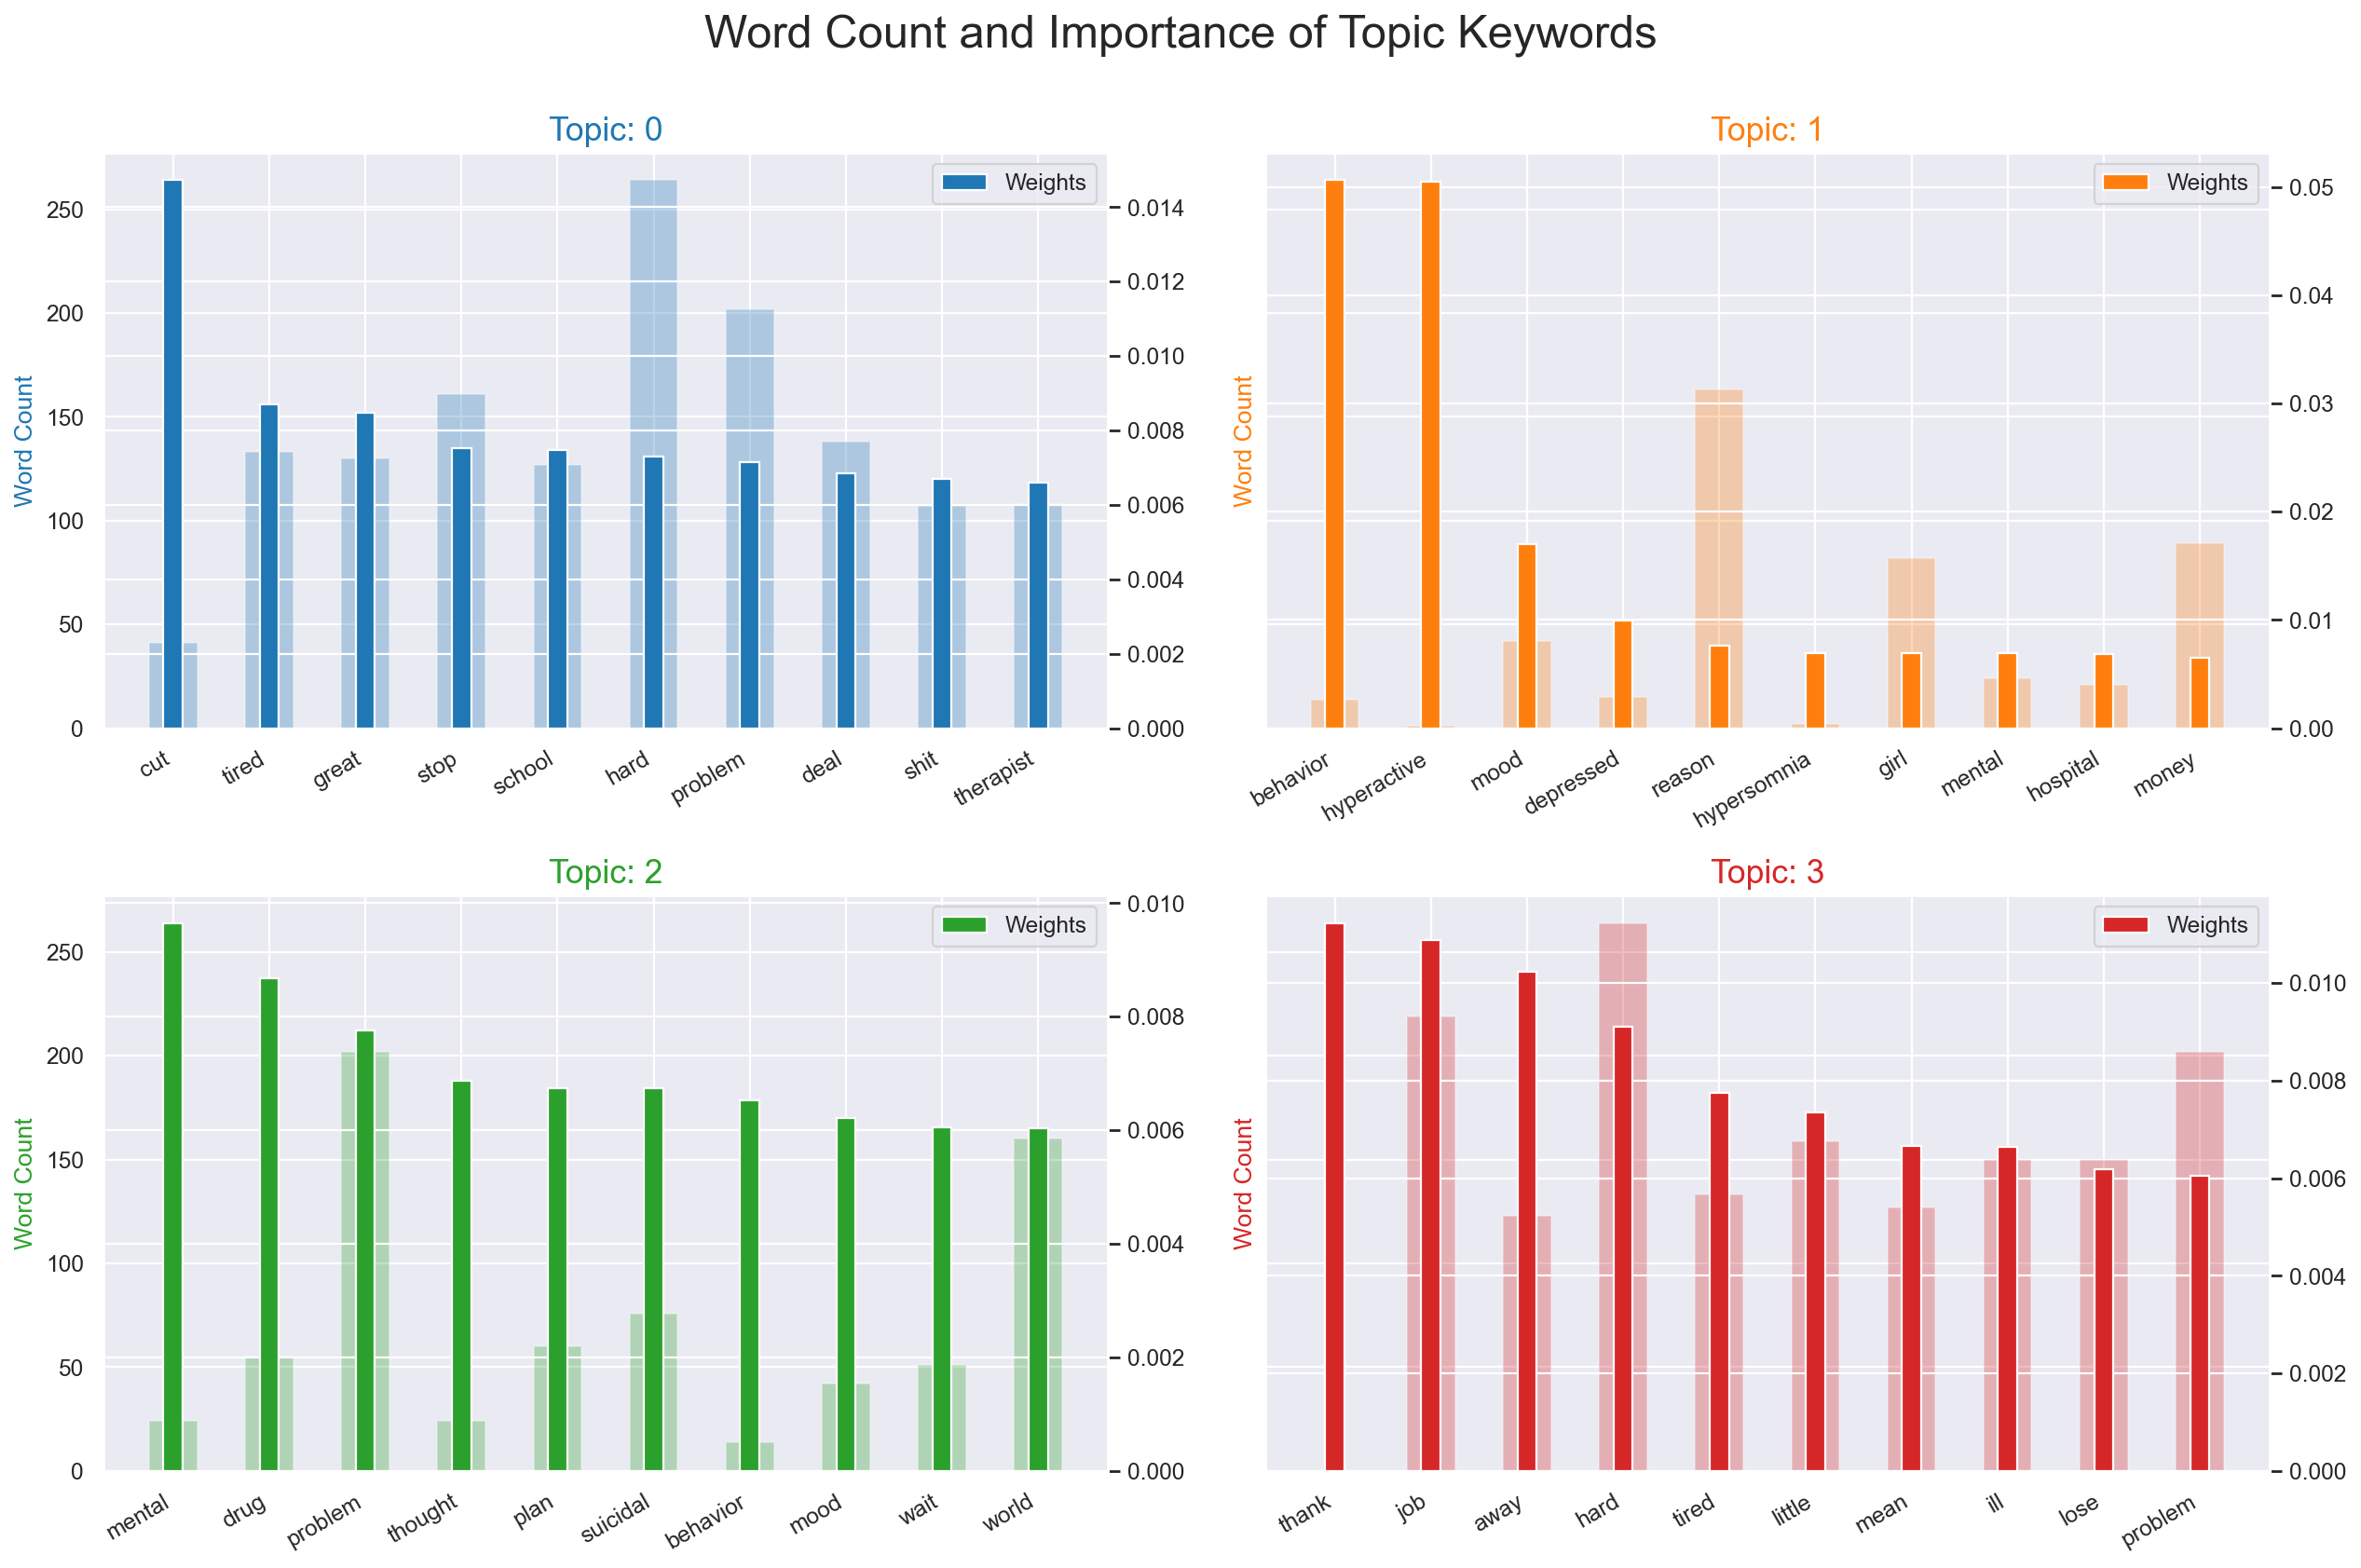
\includegraphics[width=\textwidth]{ideation_weight_relative_imp.png}
    \caption{Ideation category frequency vs LDA based relative Importance}
    \label{twitterdist}
\end{figure}  


\begin{figure}[H]
    \includegraphics[width=\textwidth]{behavior_weight_relative_imp.png}
    \caption{Behavior category frequency vs LDA based relative Importance}
    \label{redditdist}
\end{figure}


\hfill
\begin{figure}[H]
    \includegraphics[width=\textwidth]{attempt_weight_relative_imp.png}
    \caption{Attempt category frequency vs LDA based relative Importance}
    \label{twitterdist}
\end{figure}   


\subsubsection{LDA based feature exploration}
LDA is a versatile tool to investigate various keywords in subtle topic within context. LDA driven results are included in this study to observe the latent topic and terms. 

%\begin{figure}[h!]
%\centering
%\begin{subfigure}{0.45\textwidth}
%    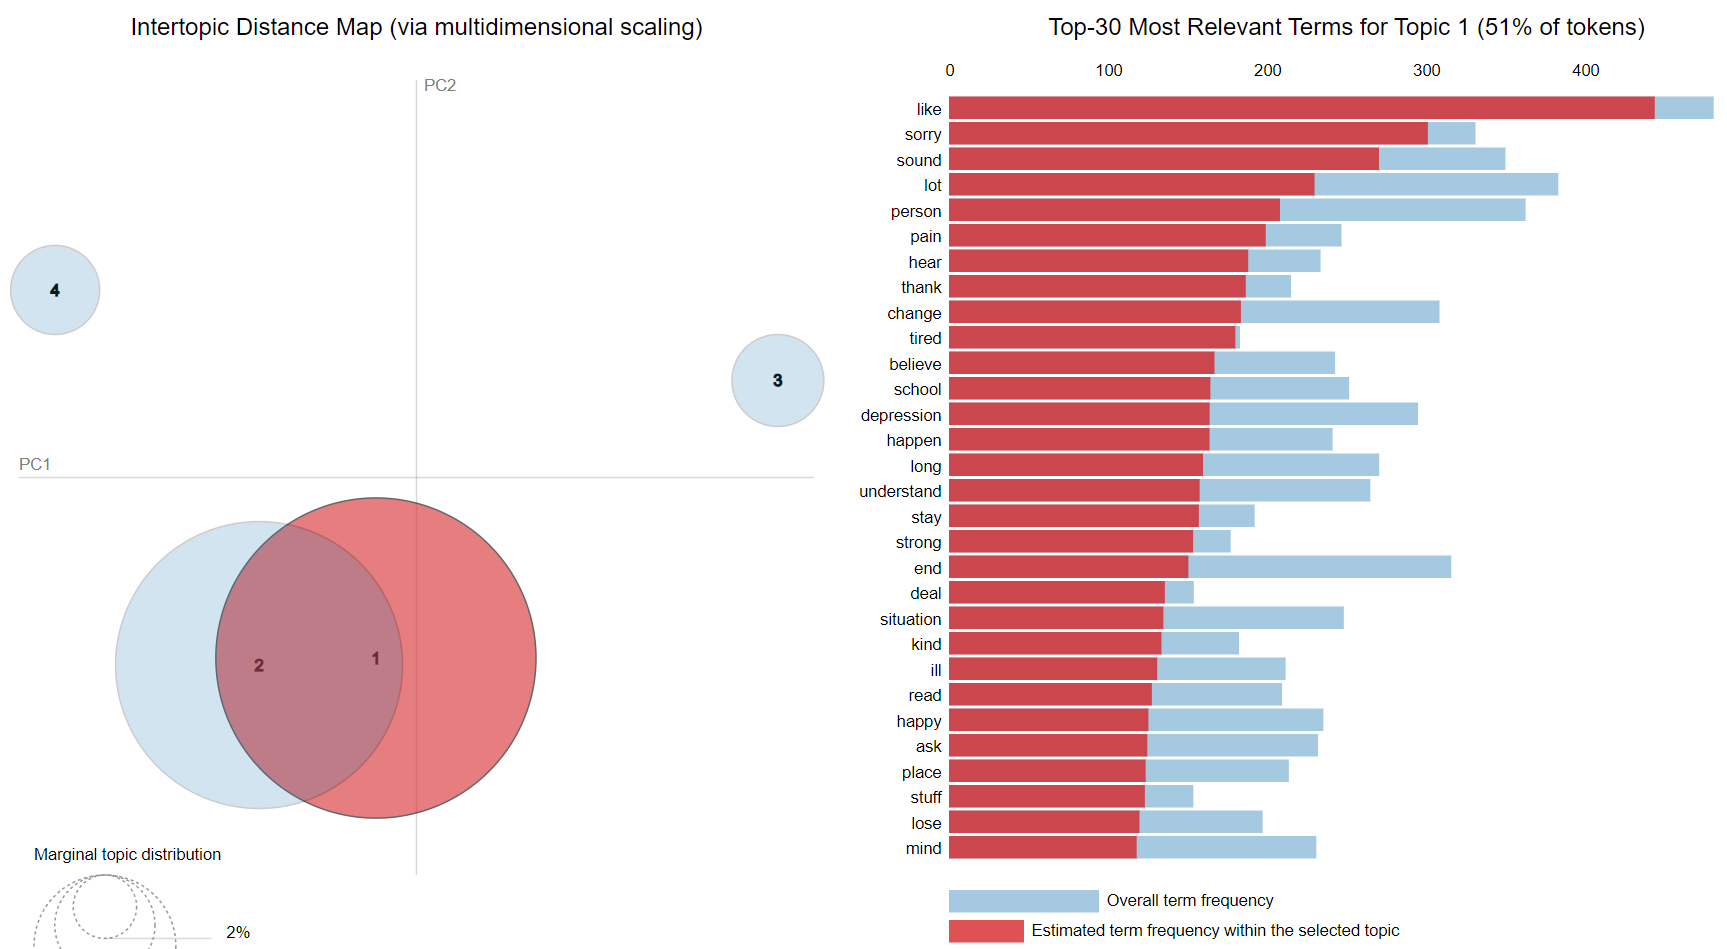
\includegraphics[width=\textwidth]{indicator_pyldvis.png}
%%    \caption{Indicator category word cloud}
%    \label{redditdist}
%\end{subfigure}
%\hfill
%\begin{subfigure}{0.45\textwidth}
%    \includegraphics[width=\textwidth]{Behavior_pyldvis.png}
%%    \caption{Behavior category word cloud}
%    \label{twitterdist}
%\end{subfigure}      
%\centering
%\begin{subfigure}{0.45\textwidth}
%    \includegraphics[width=\textwidth]{Ideation_pyldvis.png}
%%    \caption{Ideation category word cloud}
%    \label{redditdist}
%\end{subfigure}
%\hfill
%\begin{subfigure}{0.45\textwidth}
%    \includegraphics[width=\textwidth]{Attempt_pyldvis.png}
%%    \caption{Attempt category word cloud}
%    \label{twitterdist}
%\end{subfigure}   
%\caption{Inter distance topic similarities}
%\label{redditdist_twitterdist}
%\end{figure}


\begin{figure}[h!]
\centering
    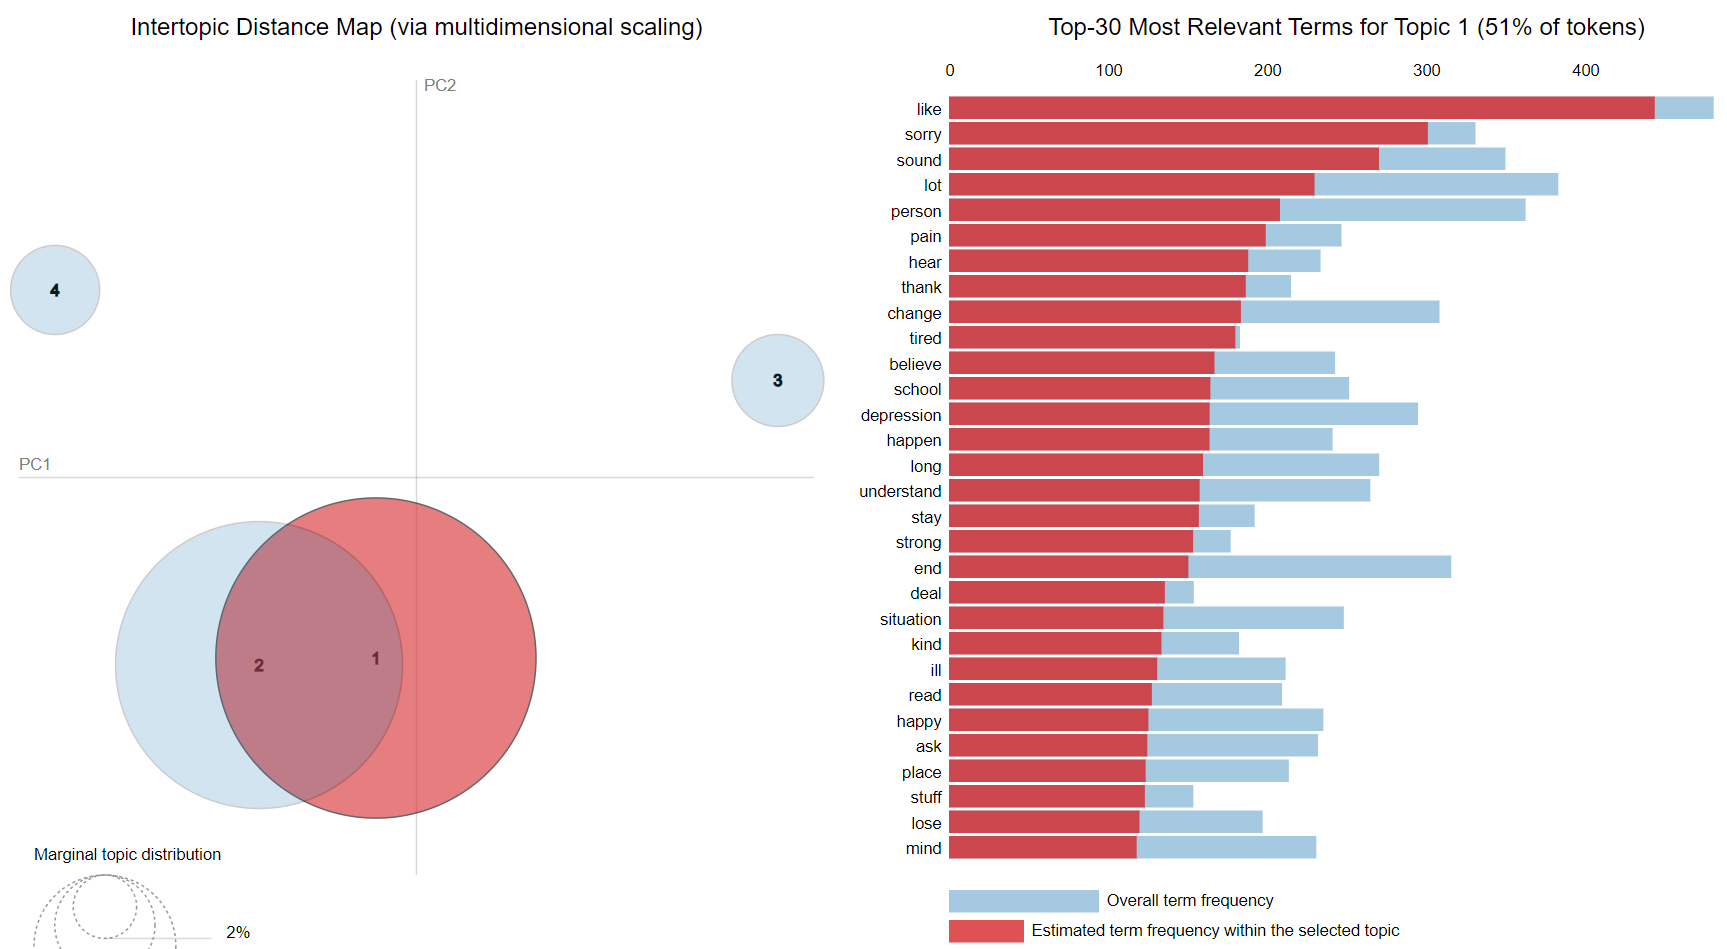
\includegraphics[width=\textwidth]{indicator_pyldvis.png}
    \caption{Indicator categories LDA's salient terms and topic visualization}
    \label{redditdist}
\end{figure}

\begin{figure}[h!]
    \includegraphics[width=\textwidth]{Ideation_pyldvis.png}
    \caption{Ideation categories LDA's salient terms and topic visualization}
    \label{redditdist}
\end{figure}

\begin{figure}[h!]
    \includegraphics[width=\textwidth]{Behavior_pyldvis.png}
    \caption{Behavior categories LDA's salient terms and topic visualization}
    \label{twitterdist}
\end{figure}

\begin{figure}[h!]
    \includegraphics[width=\textwidth]{Attempt_pyldvis.png}
    \caption{Attempt categories LDA's salient terms and topic visualization}
    \label{twitterdist}
\end{figure}


\subsubsection{Combined topic modeling using BERTopic}


\begin{figure}[h!]
\centering
\begin{subfigure}{0.45\textwidth}
    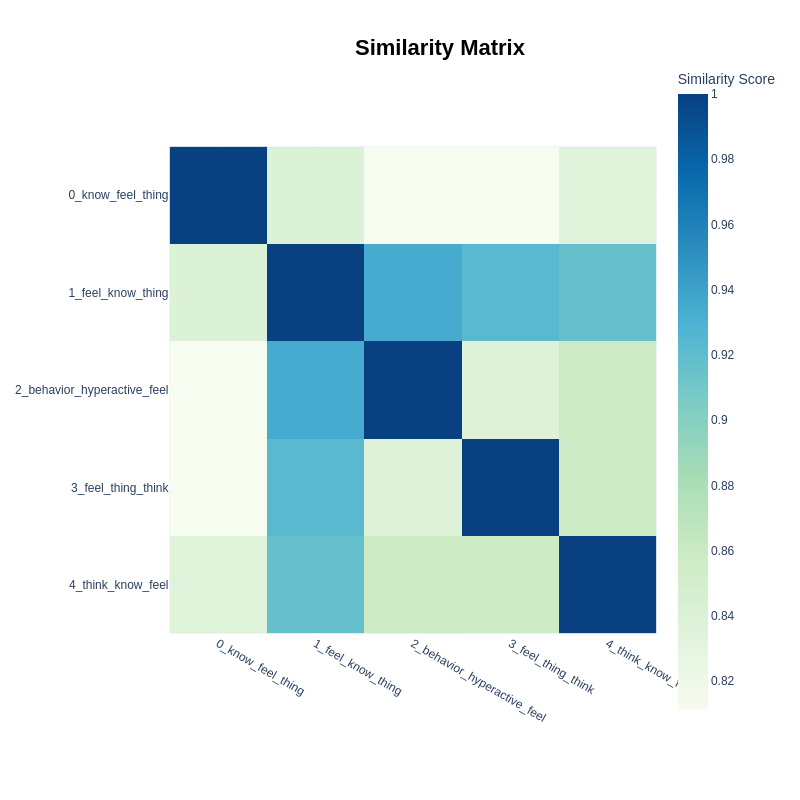
\includegraphics[width=\textwidth]{bertopic/combined_bertopic_topics_heatmap_frequency.png}
%    \caption{Ideation category word cloud}
    \label{redditdist}
\end{subfigure}
\hfill
\begin{subfigure}{0.45\textwidth}
    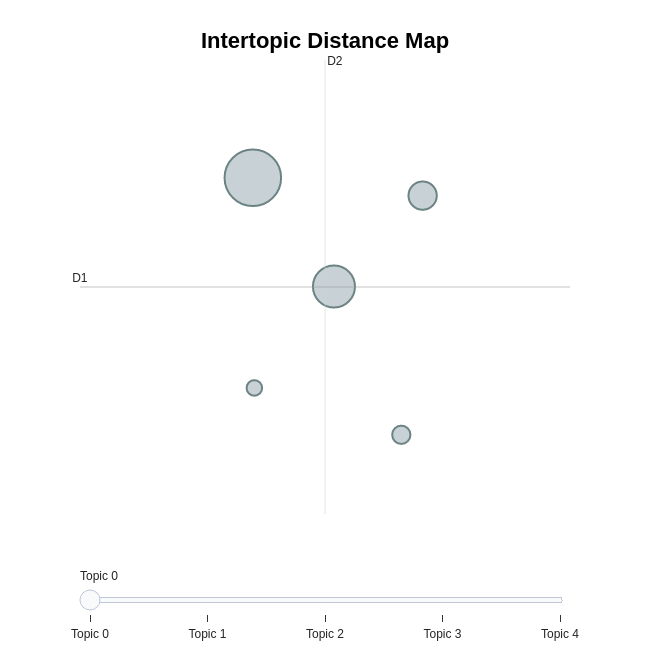
\includegraphics[width=\textwidth]{bertopic/combined_bertopic_topics_map_frequency.png}
%    \caption{Attempt category word cloud}
    \label{twitterdist}
\end{subfigure}   
\caption{Inter distance topic similarities}
\label{redditdist_twitterdist}
\end{figure}




\subsubsection{Classification}
Machine learning and Deep Learning models are particularly used for Text classification and ML for feature selection or extraction in several studies \cite{castillo2020suicide, chancellor2020methods, zhang2022natural}. These extensive reviews reveal Deep learning methods receive more attention and perform better than traditional machine learning methods whereas in some cases when extracted or filtered features are fit into training process models are able to perform better. NLP techniques are applied for the annotated dataset collected from Twitter, Reddit, Facebook, instagram, Weibo \cite{wang2020depression} etc. After that various deep learning and machine learning models are trained for classification of suicide and depression. Then trained models are applied to determine the correct class of given text. \cite{malhotra2022deep} Provided a through investigation about passed research techniques, features, datasets, and performance metrics \cite{zhang2022natural, chancellor2020methods}. 

\subsubsection{Data Learning Models}
Among Several Deep Learning approaches most successful NLP classifier for segregating Depression and suicidal task are CNN, LSTM, GRU, XLNET, BERT, Variants of BERT RoBERTa and variants of CNN such as: CNN-BiLSTM etc \cite{aldhyani2022detecting, wang2020depression, shetty2020predicting} also showed promising results. 

\subsubsection{Feature Selection} 
The feature selection procedure has a substantial impact on the performance of machine learning and deep learning models because it lowers noise in the trained dataset, enabling the model to accurately understand data patterns. LIWC, LDA, LSA, n-gram analysis \cite{pennebaker2001linguistic, tadesse2019detection} etc are used as features analysis tools. 
Most dominant approaches are n-gram word frequency based approach TF-IDF. Apart from the Deep learning model n-gram Traditional feature retrieve based analysis conducted in some research papers. In 2017 Shen et. al \cite{harvesting_social_media} collected several forms of features comprised of six chorots, namely, social network features, user profile features, visual features, emotional features, topic-level features, and domain-specific features and prepared a feature rich dictionary. This multimodal depressive dictionary learning model was used to detect the depressed users on Twitter using machine learning models. 

Most dominant approaches are Word2Vec, XGBoost, SVM, Random Forest, other regression MLs. Typical word embedding approaches TF-IDF and Word2Vec, and CNN–BiLSTM are applied in  \cite{aldhyani2022detecting}. Using LIWC features, XGBoost ML together surpasses the accuracy of CNN–BiLSTM in  \cite{aldhyani2022detecting}. Others have used machine text Summarization based feature extraction strategy followed by classification for depression detection is applied in \cite{zogan2021depressionnet}. \cite{burnap2015machine}built a set of baseline classifiers using lexical, structural, emotive and psychological features extracted from Twitter posts. Then baseline classifiers are updated by building an ensemble classifier using the Rotation Forest algorithm and a Maximum Probability voting classification decision method. \cite{chancellor2020methods} This paper provided an excellent overview of 75 studies in between 2013 and 2018 outlining the methods of data annotation for mental health status, data collection and quality management, pre-processing and feature selection, and model selection and verification. 


\section{Results Analysis}\label{sec2}
First we started our experiment with document length distribution. The length of document and term frequency within the corpus is visualized in Figure \ref{redditdist_twitterdist}. From the distribution we can see that some of the document length are excessive long and contains more than 1000 tokens ( within Twitter and also Reddit both Dataset). Depression class document length are usually shorter in length. Depression document length are tend to be smaller than suicide document length. 

Short sentence does not carry much terms and hence does not carry enough information to be classified confidently by classifier algorithms. We started reducing the numbers of samples based on document length. By reducing the samples based on numbers of tokens present in a document (see Figure \ref{redditdist_twitterdist}). Documents length versus category frequency information is showed in this chart. This charts explains if we filter out the shorter comments suicide post become dominant class and depression post become outnumbered. The difference showed an exponential pattern as length of document increases. Test dataset Reddit data distribution among depression and suicide class distribution ratio is equal. Filtering the class we have seen an interesting fact that depressed people does not want to comment very long. 





\section{Classification Results}
To segregate the Reddit suicide dataset into different categories of suicide first we have created a classifier using different classification techniques. Since our objective is not making highly accurate classifier. Following approach is applied in this study

\begin{itemize}
\item Pre-processed and useful features are used from Twitter's 500 post CSSR dataset for Training classifier
\item Used count vectorizer and TFIDF transformer to generate vectors for the dataset
\item Trained classifier to determine the categories of various suicidal intensities
\end{itemize}

We have used simple gridsearch technique of sklearn library and from a list of various classifiers applied on the dataset, we have chosen highest accurate classifiers to determine different label of suicidal risk. so that it can recognize the category. We have used classifiers "K Nearest Neighbors", "Linear and RBF SVM", "Gaussian Process", "Decision Tree", "Random Forest", "Vanilla Neural Net", "AdaBoost", "Naive Bayes". Using various set of parameters, from the result and experiments we found almost 60\% accuracy for SVM model to predict the suicide intensity categories. From various set of values of SVM we found degree=2, gamma=0.7, kernel=rbf showed the highest accuracy. 


%\begin{table}[h]
%\begin{center}
%\begin{minipage}{174pt}
%\caption{Caption text}\label{tab1}%
%\begin{tabular}{@{}lllll@{}}
%\toprule
%Classifier & Precision & Recall & Accuracy & F1 \\
%\midrule
%Nearest Neighbors & 0.926 & 0.924 & 92.3896 & 0.924\\
%RBF SVM & 0.942 & 0.924 & 92.3896 & 0.927\\
%Decision Tree & 0.901 & 0.848 & 84.7793 & 0.856\\
%Random Forest & 0.513 & 0.282 & 28.1583 & 0.167\\
%Neural Net & 0.942 & 0.927 & 92.6941 & 0.929\\
%AdaBoost & 0.905 & 0.898 & 89.8021 & 0.899\\
%Gaussian Process & 0.940 & 0.921 & 92.0852 & 0.924\\
%Naive Bayes & 0.923 & 0.918 & 91.7808 & 0.919\\
%QDA & 0.931 & 0.909 & 90.8676 & 0.912\\
%\botrule
%\end{tabular}
%\footnotetext{Shows classifiers accuracy of classification models}
%\end{minipage}
%\end{center}
%\end{table}

\subsubsection{Suicidal Intensities visualization}
How much depression can trigger suicidal thoughts is an interesting question. In this study classifier is trained on the suicidal intensity. Then trained classifier is applied on the Depression/Suicide class dataset. From various machine learning models we have found SVM is a good performing model. SVM classifier is applied for the TFIDF vectorizer embedding (see results in figure~\ref{SVMTFIDF}) and also for Word2vec pretrained vectorizer model. The results are shown in figure~\ref{Suicidal_int_vis}. From the results we can see that suicidal ideation between depression and suicidal categories number of samples are very similar. Within depression more number of samples are showed suicidal indicator category compared to suicide which is an interesting result. Suicidal behavior and attempt is comparatively high within the suicidal category than depression. Hence, figure~\ref{SVMTFIDF} result seems to be pretty obvious, except for suicidal ideation category. Also for the suicidal indicator symptoms are higher within the depression category. 

\begin{figure}[H]
\centering
\begin{subfigure}{0.45\textwidth}
    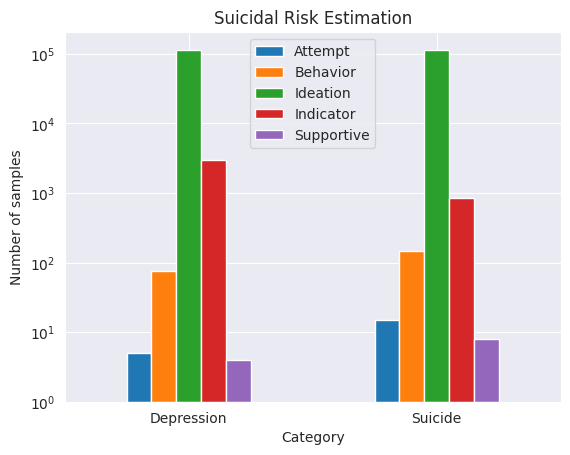
\includegraphics[width=\textwidth]{grid_svm.png}
    \caption{SVM classifier applied for TFIDF vectorizer}
    \label{SVMTFIDF}
\end{subfigure}
\hfill
\begin{subfigure}{0.45\textwidth}
    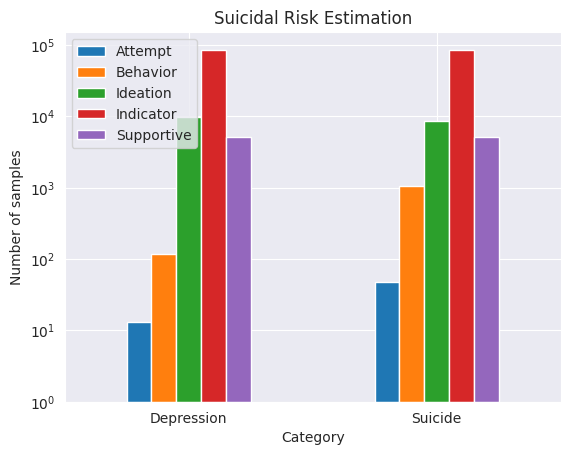
\includegraphics[width=\textwidth]{glove_vec.png}
    \caption{SVM classifier applied for Glove Word2Vec Pretrained model vectorizer}
    \label{GloveWord2Vec}
\end{subfigure}        
\caption{Visualizing suicide intensities within Depression/Suicide class}
\label{Suicidal_int_vis} 
\end{figure}

For the word2vec vector embedding scenario supportive and indicator categories results are almost similar in depression or suicide both classes. There is slight difference is shown for suicidal ideation and within suicide class, suicidal ideation is slight higher. Except the behavior and attempt category for the rest categories depression and suicide showed almost similar number of samples. 

%\begin{figure}[H]
%\centering
%\begin{subfigure}{0.45\textwidth}
%    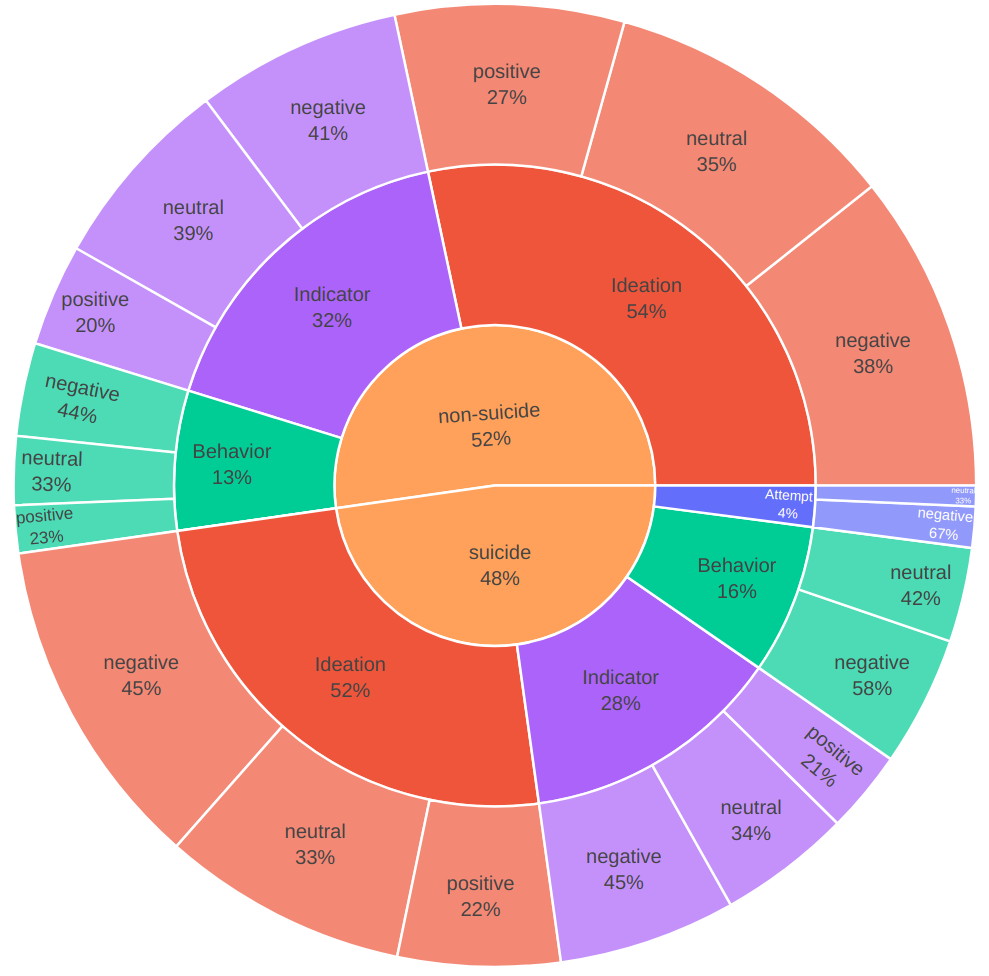
\includegraphics[width=\textwidth]{sentiment_sunburst.png}
%    \caption{First subfigure.}
%    \label{fig:first}
%\end{subfigure}
%\hfill
%\begin{subfigure}{0.45\textwidth}
%    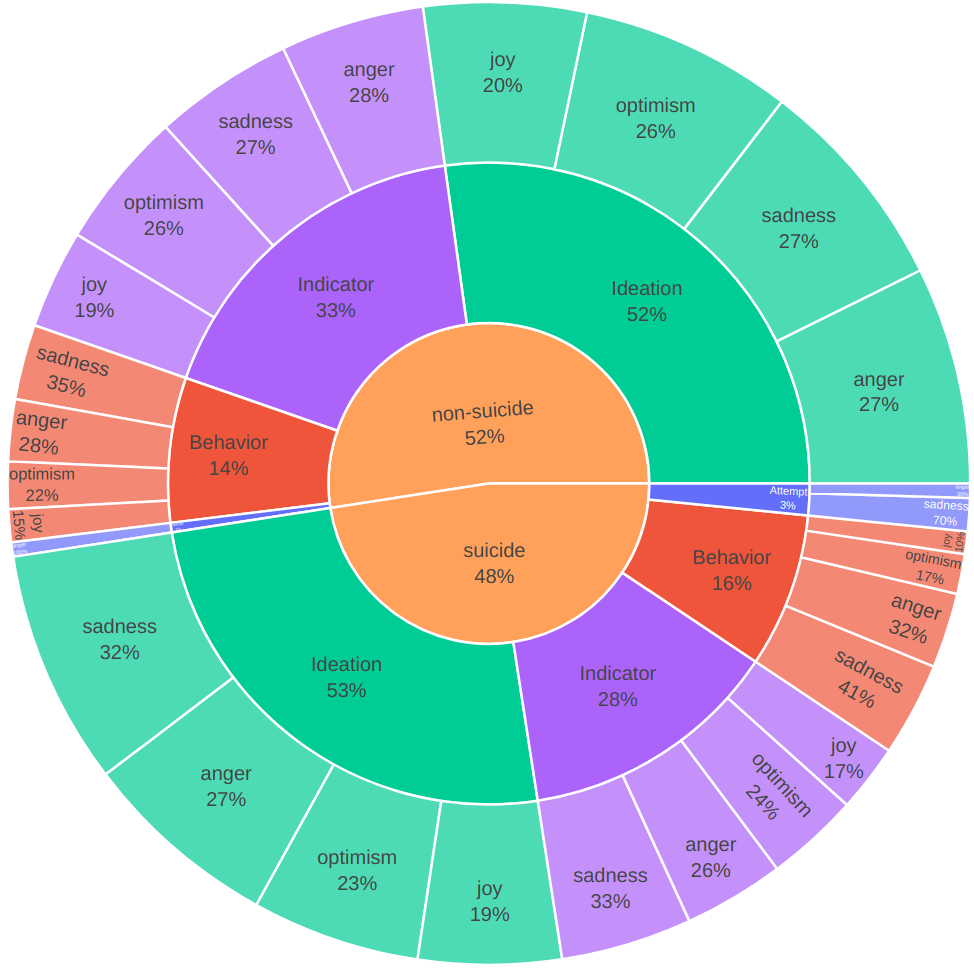
\includegraphics[width=\textwidth]{emotion_sunburst.png}
%    \caption{Second subfigure.}
%    \label{fig:second}
%\end{subfigure}
%        
%\caption{Subreferences in \LaTeX.}
%\label{fig:figures}
%\end{figure}
\section{Discussion} 
From the result it is revealed that suicide categories shown within depression and suicide class vividly. Specially suicidal ideation, indicator showed similar patterns. The number of samples within depression and suicide is almost similar for this two categories. Hence, we can infer depressed person comments showed suicidal ideation and suicidal indicating symptoms. Suicidal behavior and attempt showed higher number of samples within the suicide category compared to depression category. All these results seems very logical results. Although from the results mathematical formulas are not derived in this research study since results are susceptible to chosen classifier, chosen dataset, pretrained models vectors or embedding provided to the classifier. 
 
\section{Conclusion}
Suicidal risk estimation task and classification samples to determine suicidal risk within social websites and blogs, techniques are discussed before. According to suicidal category previous work has been done before. However, to what extent depression level triggers suicidal risk is not yet discussed before. Also it is difficult to determine since depression and suicide categorical variables are independent factor. There is not any underlying correlation. Several research conducted to segregate which post is suicidal and which one is depression various classifiers are proposed. Extensive work has been done to improve the classification accuracy by adopting most powerful vectorization techniques that uses cutting edge NLP models BERT and its various variants. Research has also been conducted on how much severity label of suicide within a post is studied. 

%\section{This is an example for first level head---section head}\label{sec3}
%
%\subsection{This is an example for second level head---subsection head}\label{subsec2}
%
%\subsubsection{This is an example for third level head---subsubsection head}\label{subsubsec2}
%
%Sample body text. Sample body text. Sample body text. Sample body text. Sample body text. Sample body text. Sample body text. Sample body text. 
%
%\section{Equations}\label{sec4}
%
%Equations in \LaTeX\ can either be inline or on-a-line by itself (``display equations''). For
%inline equations use the \verb+$...$+ commands. E.g.: The equation
%$H\psi = E \psi$ is written via the command \verb+$H \psi = E \psi$+.
%
%For display equations (with auto generated equation numbers)
%one can use the equation or align environments:
%\begin{equation}
%\|\tilde{X}(k)\|^2 \leq\frac{\sum\limits_{i=1}^{p}\left\|\tilde{Y}_i(k)\right\|^2+\sum\limits_{j=1}^{q}\left\|\tilde{Z}_j(k)\right\|^2 }{p+q}.\label{eq1}
%\end{equation}
%where,
%\begin{align}
%D_\mu &=  \partial_\mu - ig \frac{\lambda^a}{2} A^a_\mu \nonumber \\
%F^a_{\mu\nu} &= \partial_\mu A^a_\nu - \partial_\nu A^a_\mu + g f^{abc} A^b_\mu A^a_\nu \label{eq2}
%\end{align}
%Notice the use of \verb+\nonumber+ in the align environment at the end
%of each line, except the last, so as not to produce equation numbers on
%lines where no equation numbers are required. The \verb+\label{}+ command
%should only be used at the last line of an align environment where
%\verb+\nonumber+ is not used.
%\begin{equation}
%Y_\infty = \left( \frac{m}{\textrm{GeV}} \right)^{-3}
%    \left[ 1 + \frac{3 \ln(m/\textrm{GeV})}{15}
%    + \frac{\ln(c_2/5)}{15} \right]
%\end{equation}
%The class file also supports the use of \verb+\mathbb{}+, \verb+\mathscr{}+ and
%\verb+\mathcal{}+ commands. As such \verb+\mathbb{R}+, \verb+\mathscr{R}+
%and \verb+\mathcal{R}+ produces $\mathbb{R}$, $\mathscr{R}$ and $\mathcal{R}$
%respectively (refer Subsubsection~\ref{subsubsec2}).
%
%\section{Tables}\label{sec5}
%
%Tables can be inserted via the normal table and tabular environment. To put
%footnotes inside tables you should use \verb+\footnotetext[]{...}+ tag.
%The footnote appears just below the table itself (refer Tables~\ref{tab1} and \ref{tab2}). 
%For the corresponding footnotemark use \verb+\footnotemark[...]+
%


\noindent
The input format for the above table is as follows:



%%=============================================%%
%% For presentation purpose, we have included  %%
%% \bigskip command. please ignore this.       %%
%%=============================================%%

%%=============================================%%
%%% For presentation purpose, we have included  %%
%%% \bigskip command. please ignore this.       %%
%%%=============================================%%
%
%\begin{table}[h]
%\begin{center}
%\begin{minipage}{\textwidth}
%\caption{Example of a lengthy table which is set to full textwidth}\label{tab2}
%\begin{tabular*}{\textwidth}{@{\extracolsep{\fill}}lcccccc@{\extracolsep{\fill}}}
%\toprule%
%& \multicolumn{3}{@{}c@{}}{Element 1\footnotemark[1]} & \multicolumn{3}{@{}c@{}}{Element 2\footnotemark[2]} \\\cmidrule{2-4}\cmidrule{5-7}%
%Project & Energy & $\sigma_{calc}$ & $\sigma_{expt}$ & Energy & $\sigma_{calc}$ & $\sigma_{expt}$ \\
%\midrule
%Element 3  & 990 A & 1168 & $1547\pm12$ & 780 A & 1166 & $1239\pm100$\\
%Element 4  & 500 A & 961  & $922\pm10$  & 900 A & 1268 & $1092\pm40$\\
%\botrule
%\end{tabular*}
%\footnotetext{Note: This is an example of table footnote. This is an example of table footnote this is an example of table footnote this is an example of~table footnote this is an example of table footnote.}
%\footnotetext[1]{Example for a first table footnote.}
%\footnotetext[2]{Example for a second table footnote.}
%\end{minipage}
%\end{center}
%\end{table}
%
%In case of double column layout, tables which do not fit in single column width should be set to full text width. For this, you need to use \verb+\begin{table*}+ \verb+...+ \verb+\end{table*}+ instead of \verb+\begin{table}+ \verb+...+ \verb+\end{table}+ environment. Lengthy tables which do not fit in textwidth should be set as rotated table. For this, you need to use \verb+\begin{sidewaystable}+ \verb+...+ \verb+\end{sidewaystable}+ instead of \verb+\begin{table*}+ \verb+...+ \verb+\end{table*}+ environment. This environment puts tables rotated to single column width. For tables rotated to double column width, use \verb+\begin{sidewaystable*}+ \verb+...+ \verb+\end{sidewaystable*}+.
%
%\begin{sidewaystable}
%\sidewaystablefn%
%\begin{center}
%\begin{minipage}{\textheight}
%\caption{Tables which are too long to fit, should be written using the ``sidewaystable'' environment as shown here}\label{tab3}
%\begin{tabular*}{\textheight}{@{\extracolsep{\fill}}lcccccc@{\extracolsep{\fill}}}
%\toprule%
%& \multicolumn{3}{@{}c@{}}{Element 1\footnotemark[1]}& \multicolumn{3}{@{}c@{}}{Element\footnotemark[2]} \\\cmidrule{2-4}\cmidrule{5-7}%
%Projectile & Energy	& $\sigma_{calc}$ & $\sigma_{expt}$ & Energy & $\sigma_{calc}$ & $\sigma_{expt}$ \\
%\midrule
%Element 3 & 990 A & 1168 & $1547\pm12$ & 780 A & 1166 & $1239\pm100$ \\
%Element 4 & 500 A & 961  & $922\pm10$  & 900 A & 1268 & $1092\pm40$ \\
%Element 5 & 990 A & 1168 & $1547\pm12$ & 780 A & 1166 & $1239\pm100$ \\
%Element 6 & 500 A & 961  & $922\pm10$  & 900 A & 1268 & $1092\pm40$ \\
%\botrule
%\end{tabular*}
%\footnotetext{Note: This is an example of table footnote this is an example of table footnote this is an example of table footnote this is an example of~table footnote this is an example of table footnote.}
%\footnotetext[1]{This is an example of table footnote.}
%\end{minipage}
%\end{center}
%\end{sidewaystable}
%
%\section{Figures}\label{sec6}
%
%As per the \LaTeX\ standards you need to use eps images for \LaTeX\ compilation and \verb+pdf/jpg/png+ images for \verb+PDFLaTeX+ compilation. This is one of the major difference between \LaTeX\ and \verb+PDFLaTeX+. Each image should be from a single input .eps/vector image file. Avoid using subfigures. The command for inserting images for \LaTeX\ and \verb+PDFLaTeX+ can be generalized. The package used to insert images in \verb+LaTeX/PDFLaTeX+ is the graphicx package. Figures can be inserted via the normal figure environment as shown in the below example:
%
%%%=============================================%%
%%% For presentation purpose, we have included  %%
%%% \bigskip command. please ignore this.       %%
%%%=============================================%%
%\bigskip
%\begin{verbatim}
%\begin{figure}[<placement-specifier>]
%\centering
%\includegraphics{<eps-file>}
%\caption{<figure-caption>}\label{<figure-label>}
%\end{figure}
%\end{verbatim}
%\bigskip
%%%=============================================%%
%%% For presentation purpose, we have included  %%
%%% \bigskip command. please ignore this.       %%
%%%=============================================%%
%
%\begin{figure}[h]%
%\centering
%
\includegraphics[width=0.9\textwidth]{fig.eps}
%\caption{This is a widefig. This is an example of long caption this is an example of long caption  this is an example of long caption this is an example of long caption}\label{fig1}
%\end{figure}
%
%In case of double column layout, the above format puts figure captions/images to single column width. To get spanned images, we need to provide \verb+\begin{figure*}+ \verb+...+ \verb+\end{figure*}+.
%
%For sample purpose, we have included the width of images in the optional argument of \verb+\includegraphics+ tag. Please ignore this. 
%
%\section{Algorithms, Program codes and Listings}\label{sec7}
%
%Packages \verb+algorithm+, \verb+algorithmicx+ and \verb+algpseudocode+ are used for setting algorithms in \LaTeX\ using the format:
%
%%%=============================================%%
%%% For presentation purpose, we have included  %%
%%% \bigskip command. please ignore this.       %%
%%%=============================================%%
%\bigskip
%\begin{verbatim}
%\begin{algorithm}
%\caption{<alg-caption>}\label{<alg-label>}
%\begin{algorithmic}[1]
%. . .
%\end{algorithmic}
%\end{algorithm}
%\end{verbatim}
%\bigskip
%%%=============================================%%
%%% For presentation purpose, we have included  %%
%%% \bigskip command. please ignore this.       %%
%%%=============================================%%
%
%You may refer above listed package documentations for more details before setting \verb+algorithm+ environment. For program codes, the ``program'' package is required and the command to be used is \verb+\begin{program}+ \verb+...+ \verb+\end{program}+. A fast exponentiation procedure:
%
%\begin{program}
%\BEGIN \\ %
%  \FOR i:=1 \TO 10 \STEP 1 \DO
%     |expt|(2,i); \\ |newline|() \OD %
%\rcomment{Comments will be set flush to the right margin}
%\WHERE
%\PROC |expt|(x,n) \BODY
%          z:=1;
%          \DO \IF n=0 \THEN \EXIT \FI;
%             \DO \IF |odd|(n) \THEN \EXIT \FI;
%\COMMENT{This is a comment statement};
%                n:=n/2; x:=x*x \OD;
%             \{ n>0 \};
%             n:=n-1; z:=z*x \OD;
%          |print|(z) \ENDPROC
%\END
%\end{program}
%
%
%\begin{algorithm}
%\caption{Calculate $y = x^n$}\label{algo1}
%\begin{algorithmic}[1]
%\Require $n \geq 0 \vee x \neq 0$
%\Ensure $y = x^n$ 
%\State $y \Leftarrow 1$
%\If{$n < 0$}\label{algln2}
%        \State $X \Leftarrow 1 / x$
%        \State $N \Leftarrow -n$
%\Else
%        \State $X \Leftarrow x$
%        \State $N \Leftarrow n$
%\EndIf
%\While{$N \neq 0$}
%        \If{$N$ is even}
%            \State $X \Leftarrow X \times X$
%            \State $N \Leftarrow N / 2$
%        \Else[$N$ is odd]
%            \State $y \Leftarrow y \times X$
%            \State $N \Leftarrow N - 1$
%        \EndIf
%\EndWhile
%\end{algorithmic}
%\end{algorithm}
%\bigskip
%%%=============================================%%
%%% For presentation purpose, we have included  %%
%%% \bigskip command. please ignore this.       %%
%%%=============================================%%
%
%Similarly, for \verb+listings+, use the \verb+listings+ package. \verb+\begin{lstlisting}+ \verb+...+ \verb+\end{lstlisting}+ is used to set environments similar to \verb+verbatim+ environment. Refer to the \verb+lstlisting+ package documentation for more details.
%
%%%=============================================%%
%%% For presentation purpose, we have included  %%
%%% \bigskip command. please ignore this.       %%
%%%=============================================%%
%\bigskip
%\begin{minipage}{\hsize}%
%\lstset{frame=single,framexleftmargin=-1pt,framexrightmargin=-17pt,framesep=12pt,linewidth=0.98\textwidth,language=pascal}% Set your language (you can change the language for each code-block optionally)
%%%% Start your code-block
%\begin{lstlisting}
%for i:=maxint to 0 do
%begin
%{ do nothing }
%end;
%Write('Case insensitive ');
%Write('Pascal keywords.');
%\end{lstlisting}
%\end{minipage}
%
%\section{Cross referencing}\label{sec8}
%
%Environments such as figure, table, equation and align can have a label
%declared via the \verb+\label{#label}+ command. For figures and table
%environments use the \verb+\label{}+ command inside or just
%below the \verb+\caption{}+ command. You can then use the
%\verb+\ref{#label}+ command to cross-reference them. As an example, consider
%the label declared for Figure~\ref{fig1} which is
%\verb+\label{fig1}+. To cross-reference it, use the command 
%\verb+Figure \ref{fig1}+, for which it comes up as
%``Figure~\ref{fig1}''. 
%
%To reference line numbers in an algorithm, consider the label declared for the line number 2 of Algorithm~\ref{algo1} is \verb+\label{algln2}+. To cross-reference it, use the command \verb+\ref{algln2}+ for which it comes up as line~\ref{algln2} of Algorithm~\ref{algo1}.
%
%\subsection{Details on reference citations}\label{subsec7}
%
%Standard \LaTeX\ permits only numerical citations. To support both numerical and author-year citations this template uses \verb+natbib+ \LaTeX\ package. For style guidance please refer to the template user manual.
%
%Here is an example for \verb+\cite{...}+: \cite{bib1}. Another example for \verb+\citep{...}+: \citep{bib2}. For author-year citation mode, \verb+\cite{...}+ prints Jones et al. (1990) and \verb+\citep{...}+ prints (Jones et al., 1990).
%
%All cited bib entries are printed at the end of this article: \cite{bib3}, \cite{bib4}, \cite{bib5}, \cite{bib6}, \cite{bib7}, \cite{bib8}, \cite{bib9}, \cite{bib10}, \cite{bib11} and \cite{bib12}.
%
%\section{Examples for theorem like environments}\label{sec10}
%
%For theorem like environments, we require \verb+amsthm+ package. There are three types of predefined theorem styles exists---\verb+thmstyleone+, \verb+thmstyletwo+ and \verb+thmstylethree+ 
%
%%%=============================================%%
%%% For presentation purpose, we have included  %%
%%% \bigskip command. please ignore this.       %%
%%%=============================================%%
%\bigskip
%\begin{tabular}{|l|p{19pc}|}
%\hline
%\verb+thmstyleone+ & Numbered, theorem head in bold font and theorem text in italic style \\\hline
%\verb+thmstyletwo+ & Numbered, theorem head in roman font and theorem text in italic style \\\hline
%\verb+thmstylethree+ & Numbered, theorem head in bold font and theorem text in roman style \\\hline
%\end{tabular}
%\bigskip
%%%=============================================%%
%%% For presentation purpose, we have included  %%
%%% \bigskip command. please ignore this.       %%
%%%=============================================%%
%
%For mathematics journals, theorem styles can be included as shown in the following examples:
%
%\begin{theorem}[Theorem subhead]\label{thm1}
%Example theorem text. Example theorem text. Example theorem text. Example theorem text. Example theorem text. 
%Example theorem text. Example theorem text. Example theorem text. Example theorem text. Example theorem text. 
%Example theorem text. 
%\end{theorem}
%
%Sample body text. Sample body text. Sample body text. Sample body text. Sample body text. Sample body text. Sample body text. Sample body text.
%
%\begin{proposition}
%Example proposition text. Example proposition text. Example proposition text. Example proposition text. Example proposition text. 
%Example proposition text. Example proposition text. Example proposition text. Example proposition text. Example proposition text. 
%\end{proposition}
%
%Sample body text. Sample body text. Sample body text. Sample body text. Sample body text. Sample body text. Sample body text. Sample body text.
%
%\begin{example}
%Phasellus adipiscing semper elit. Proin fermentum massa
%ac quam. Sed diam turpis, molestie vitae, placerat a, molestie nec, leo. Maecenas lacinia. Nam ipsum ligula, eleifend
%at, accumsan nec, suscipit a, ipsum. Morbi blandit ligula feugiat magna. Nunc eleifend consequat lorem. 
%\end{example}
%
%Sample body text. Sample body text. Sample body text. Sample body text. Sample body text. Sample body text. Sample body text. Sample body text.
%
%\begin{remark}
%Phasellus adipiscing semper elit. Proin fermentum massa
%ac quam. Sed diam turpis, molestie vitae, placerat a, molestie nec, leo. Maecenas lacinia. Nam ipsum ligula, eleifend
%at, accumsan nec, suscipit a, ipsum. Morbi blandit ligula feugiat magna. Nunc eleifend consequat lorem. 
%\end{remark}
%
%Sample body text. Sample body text. Sample body text. Sample body text. Sample body text. Sample body text. Sample body text. Sample body text.
%
%\begin{definition}[Definition sub head]
%Example definition text. Example definition text. Example definition text. Example definition text. Example definition text. Example definition text. Example definition text. Example definition text. 
%\end{definition}
%
%Additionally a predefined ``proof'' environment is available: \verb+\begin{proof}+ \verb+...+ \verb+\end{proof}+. This prints a ``Proof'' head in italic font style and the ``body text'' in roman font style with an open square at the end of each proof environment. 
%
%\begin{proof}
%Example for proof text. Example for proof text. Example for proof text. Example for proof text. Example for proof text. Example for proof text. Example for proof text. Example for proof text. Example for proof text. Example for proof text. 
%\end{proof}
%
%Sample body text. Sample body text. Sample body text. Sample body text. Sample body text. Sample body text. Sample body text. Sample body text.
%
%\begin{proof}[Proof of Theorem~{\upshape\ref{thm1}}]
%Example for proof text. Example for proof text. Example for proof text. Example for proof text. Example for proof text. Example for proof text. Example for proof text. Example for proof text. Example for proof text. Example for proof text. 
%\end{proof}
%
%\noindent
%For a quote environment, use \verb+\begin{quote}...\end{quote}+
%\begin{quote}
%Quoted text example. Aliquam porttitor quam a lacus. Praesent vel arcu ut tortor cursus volutpat. In vitae pede quis diam bibendum placerat. Fusce elementum
%convallis neque. Sed dolor orci, scelerisque ac, dapibus nec, ultricies ut, mi. Duis nec dui quis leo sagittis commodo.
%\end{quote}
%
%Sample body text. Sample body text. Sample body text. Sample body text. Sample body text (refer Figure~\ref{fig1}). Sample body text. Sample body text. Sample body text (refer Table~\ref{tab3}). 
%
%\section{Methods}\label{sec11}
%
%Topical subheadings are allowed. Authors must ensure that their Methods section includes adequate experimental and characterization data necessary for others in the field to reproduce their work. Authors are encouraged to include RIIDs where appropriate. 
%
%\textbf{Ethical approval declarations} (only required where applicable) Any article reporting experiment/s carried out on (i)~live vertebrate (or higher invertebrates), (ii)~humans or (iii)~human samples must include an unambiguous statement within the methods section that meets the following requirements: 
%
%\begin{enumerate}[1.]
%\item Approval: a statement which confirms that all experimental protocols were approved by a named institutional and/or licensing committee. Please identify the approving body in the methods section
%
%\item Accordance: a statement explicitly saying that the methods were carried out in accordance with the relevant guidelines and regulations
%
%\item Informed consent (for experiments involving humans or human tissue samples): include a statement confirming that informed consent was obtained from all participants and/or their legal guardian/s
%\end{enumerate}
%
%If your manuscript includes potentially identifying patient/participant information, or if it describes human transplantation research, or if it reports results of a clinical trial then  additional information will be required. Please visit (\url{https://www.nature.com/nature-research/editorial-policies}) for Nature Portfolio journals, (\url{https://www.springer.com/gp/authors-editors/journal-author/journal-author-helpdesk/publishing-ethics/14214}) for Springer Nature journals, or (\url{https://www.biomedcentral.com/getpublished/editorial-policies\#ethics+and+consent}) for BMC.
%
%\section{Discussion}\label{sec12}
%
%Discussions should be brief and focused. In some disciplines use of Discussion or `Conclusion' is interchangeable. It is not mandatory to use both. Some journals prefer a section `Results and Discussion' followed by a section `Conclusion'. Please refer to Journal-level guidance for any specific requirements. 
%
%\section{Conclusion}\label{sec13}
%
%From the analysis we found there are strong correlation within the features among this two categories depression and suicide post. The most frequent words of two categories has similarities. After using the exploratory analysis using scatterplot we saw many words which seems to be a written post word from depressed person appears within suicide category. During analysis one interesting result is observed that depression persons post is relatively shorter and full of abusive words. Simple Term frequency based vectorization technique could not effectively estimates the depression impact. Surprisingly, after analysis with TFIDF and countvectorization methods we found that there is 99\% chance that the person who is depressed also has suicial tendency. Here, gridsearch technique is used to determine the best classification estimator. Since, vectorizer is not trained with the reddit dataset. Hence, we are assuming that after getting the result the vectors are not god enough to classify right way. Also, another reason is we compelled the classifier to classify the samples in suicidal risk categories. Hence, it does not have a choice rather than label the sample to suicidal risk category.  
%
%\backmatter
%
%\bmhead{Supplementary information}
%
%If your article has accompanying supplementary file/s please state so here. 
%
%Authors reporting data from electrophoretic gels and blots should supply the full unprocessed scans for key as part of their Supplementary information. This may be requested by the editorial team/s if it is missing.
%
%Please refer to Journal-level guidance for any specific requirements.
%
%\bmhead{Acknowledgments}
%
%Acknowledgments are not compulsory. Where included they should be brief. Grant or contribution numbers may be acknowledged.
%
%Please refer to Journal-level guidance for any specific requirements.
%
%\section*{Declarations}
%
%Some journals require declarations to be submitted in a standardised format. Please check the Instructions for Authors of the journal to which you are submitting to see if you need to complete this section. If yes, your manuscript must contain the following sections under the heading `Declarations':
%
%\begin{itemize}
%\item Funding
%\item Conflict of interest/Competing interests (check journal-specific guidelines for which heading to use)
%\item Ethics approval 
%\item Consent to participate
%\item Consent for publication
%\item Availability of data and materials
%\item Code availability 
%\item Authors' contributions
%\end{itemize}
%
%\noindent
%If any of the sections are not relevant to your manuscript, please include the heading and write `Not applicable' for that section. 
%
%%%===================================================%%
%%% For presentation purpose, we have included        %%
%%% \bigskip command. please ignore this.             %%
%%%===================================================%%
%\bigskip
%\begin{flushleft}%
%Editorial Policies for:
%
%\bigskip\noindent
%Springer journals and proceedings: \url{https://www.springer.com/gp/editorial-policies}
%
%\bigskip\noindent
%Nature Portfolio journals: \url{https://www.nature.com/nature-research/editorial-policies}
%
%\bigskip\noindent
%\textit{Scientific Reports}: \url{https://www.nature.com/srep/journal-policies/editorial-policies}
%
%\bigskip\noindent
%BMC journals: \url{https://www.biomedcentral.com/getpublished/editorial-policies}
%\end{flushleft}
%
%\begin{appendices}
%
%\section{Section title of first appendix}\label{secA1}
%
%An appendix contains supplementary information that is not an essential part of the text itself but which may be helpful in providing a more comprehensive understanding of the research problem or it is information that is too cumbersome to be included in the body of the paper.
%
%%%=============================================%%
%%% For submissions to Nature Portfolio Journals %%
%%% please use the heading ``Extended Data''.   %%
%%%=============================================%%
%
%%%=============================================================%%
%%% Sample for another appendix section			       %%
%%%=============================================================%%
%
%%% \section{Example of another appendix section}\label{secA2}%
%%% Appendices may be used for helpful, supporting or essential material that would otherwise 
%%% clutter, break up or be distracting to the text. Appendices can consist of sections, figures, 
%%% tables and equations etc.
%
%\end{appendices}
%
%%%===========================================================================================%%
%%% If you are submitting to one of the Nature Portfolio journals, using the eJP submission   %%
%%% system, please include the references within the manuscript file itself. You may do this  %%
%%% by copying the reference list from your .bbl file, paste it into the main manuscript .tex %%
%%% file, and delete the associated \verb+\bibliography+ commands.                            %%
%%%===========================================================================================%%

%\bibliography{sn-bibliography}% common bib file
%% if required, the content of .bbl file can be included here once bbl is generated
%%\input sn-article.bbl

%% Default %%
\input doc_ref.tex
%%\bibliographystyle{alpha} % We choose the "plain" reference style
%\bibliography{sn-bibliography} % Entries are in the refs.bib file

\end{document}
